%--------------------------------------------------------------------%
%
% Berkas utama templat LaTeX.
%
% author Petra Barus, Peb Ruswono Aryan
%
%--------------------------------------------------------------------%
%
% Berkas ini berisi struktur utama dokumen LaTeX yang akan dibuat.
%
%--------------------------------------------------------------------%
\documentclass[12pt, a4paper, onecolumn, oneside, final]{report}
\special{papersize=210mm,297mm}

% set margin
%\usepackage{showframe}
\usepackage[top=2.7cm,bottom=3cm,left=4cm,right=3cm]{geometry}

% set font
\usepackage{mathptmx}

% judul bahasa Indonesia
\usepackage[bahasa]{babel}

% satu setengah spasi
\renewcommand{\baselinestretch}{1.5}

\usepackage[utf8]{inputenc}

% citation style
\usepackage[backend=bibtex,citestyle=authoryear]{biblatex}

\usepackage[autostyle]{csquotes}
\usepackage{graphicx}
\usepackage{titling}
\usepackage{blindtext}
\usepackage{sectsty}
\usepackage{chngcntr}
\usepackage[table,xcdraw]{xcolor}
\usepackage{textcomp}
\usepackage{float}
\usepackage{caption}
\usepackage{tabularx}

%remove spacing before chapter
\usepackage{titlesec}
\titleformat{\chapter}[display]
{\normalfont\large\bfseries\centering}{\chaptertitlename\ \thechapter}{8pt}{\centering\large}
\titlespacing*{\chapter}{0pt}{-20pt}{40pt}

%merapikan antara nomor list dan textnya
\usepackage{tocloft}
\setlength{\cfttabnumwidth}{1.5cm}
\setlength{\cftfignumwidth}{1.5cm}

\setlength{\cftbeforetoctitleskip}{-20pt}
\renewcommand{\cfttoctitlefont}{\hfill\large\bfseries}
\renewcommand{\cftaftertoctitle}{\hfill\hfill}

\setlength{\cftbeforeloftitleskip}{-20pt}
\renewcommand{\cftloftitlefont}{\hfill\hfill\large\bfseries}
\renewcommand{\cftafterloftitle}{\hfill\hfill}

\setlength{\cftbeforelottitleskip}{-20pt}
\renewcommand{\cftlottitlefont}{\hfill\hfill\large\bfseries}
\renewcommand{\cftafterlottitle}{\hfill\hfill}

\usepackage{listings}
\lstset{breaklines=true,basicstyle=\ttfamily}

\floatstyle{plaintop}
\restylefloat{table}

\counterwithin{figure}{section}
\counterwithin{table}{section}

\captionsetup[table]{skip=10pt}
\captionsetup[figure]{name={Gambar.},labelsep=period}

\makeatletter
\def\@kampus{PROGRAM STUDI TEKNIK INFORMATIKA\\
	SEKOLAH TEKNIK ELEKTRO DAN INFORMATIKA\\
	Institut Teknologi Bandung}
%\def\@maketitle{   % custom maketitle
\newcommand{\judul}{   % custom maketitle

\begin{center}
\smallskip
\large \bfseries \thetitle
\vfill
\large Laporan Tugas Akhir\\
\vfill
Disusun sebagai syarat kelulusan tingkat sarjana\\
\vfill
oleh\\
\large \theauthor
\vfill
\begin{figure}[h]
\centering
  	\includegraphics[width=0.15\textwidth]{resources/cover-ganesha.jpg}
\end{figure}
\vfill
\large
\@kampus \\
\large
\the\year

\end{center}
}
\makeatother

\sectionfont{\normalsize}
\subsectionfont{\normalsize}

\renewcommand{\thechapter}{\Roman{chapter}}

\bibliography{references}

\begin{document}

\title{IMPLEMENTASI DPI PADA IPTABLES SEBAGAI PENANGKAL INFEKSI MALWARE MELALUI JARINGAN}
\date{}
\author{IBROHIM KHOLILUL ISLAM\\
NIM : 13513090}

\input{chapters/cover}
\LARGE
\textbf{\thetitle}
\small

\begin{center}
	
	\vfill
	\textbf{Draf Laporan Tugas Akhir II}\\
	\vfill
	oleh\\
	\theauthor
	\vfill
	Program Studi: Teknik Informatika \\
	Sekolah Teknik Elektro dan Informatika \\
	Institut Teknologi Bandung
	\vfill
	Bandung, 7 Desember 2018 \\
	Mengetahui,\\
	Pembimbing \\
	\vspace{60pt}
	Yudistira Dwi Wardhana Asnar ST, Ph.D.\\
	NIP. 19800827 201504 1 002
\end{center}

\pagenumbering{roman}
\setcounter{page}{0}

\pagestyle{plain}

\clearpage
\chapter*{ABSTRAK}
\addcontentsline{toc}{chapter}{Abstrak}

Pada tugas akhir ini, dikembangkan sebuah \textit{inline network-based malware detection} untuk melakukan deteksi malware. Hal ini dilakukan karena firewall saat ini masih belum dapat melakukan deteksi infeksi malware. Malware yang dipakai pada pengembangan ini adalah malware WannaCry yang menginfeksi lebih dari 75.000 host pada 2017. \textit{Inline network-based malware detection} diterapkan pada sebuah firewall sehingga dapat melakukan penagkalan infeksi.

Pengembangan dilakukan dengan menggunakan teknik \textit{dynamic signature-based}. Teknik ini secara teori dapat meminimalisir \textit{false-negative} dibandingkan dengan teknik \textit{anomaly-based}. Signature yang dibentuk dari hasil inspeksi oleh DPI yang dikembangkan untuk protokol SMB. Signature dalam bentuk \textit{state machine} dari hasil inspeksi oleh SMB digunakan untuk menentukan apakah sebuah paket berbahaya atau tidak.

Pengujian dilakukan dengan melakukan percobaan. Percobaan dilakukan dengan menerapkan transparent-firewall dalam sebuah subnet. Hasil percobaan menunjukan implementasi \textit{inline network-based malware detection} tersebut dapat melakukan penangkalan pada 83 percobaan yang telah dilakukan. Dalam percobaan tersebut belum menunjukan ditemukannya \textit{false-negative}. Namun pada perancangan pengujian tidak dilakukan untuk mendeteksi \textit{false-positive}.

\vspace{17px} \noindent Kata kunci: \textit{network-based malware detection}, firewall, wannacry

\clearpage
\input{chapters/abstract-en}
\chapter*{Kata Pengantar}
\addcontentsline{toc}{chapter}{Kata Pengantar}

Puji dan syukur penulis panjatkan ke hadirat Tuhan Yang Maha Esa. Berkat rahmat-Nya, penulis mampu menyelesaikan Tugas Akhir yang berjudul ‘\thetitle’. Penulis juga mengucapkan terima kasih kepada:
\begin{enumerate}
	\item Dosen pembimbing, Bapak Yudistira Dwi Wardhana Asnar yang telah meluangkan waktu untuk membimbing penulis dengan memberikan ide dan saran.
	\item Korektor, Meiliany Pranolo yang telah bersedia membantu mengidentifikasi kesalahan penulisan.
	\item Staf Prodi Teknik Informatika ITB, terutama para dosen yang telah membagikan ilmu dan tata usaha yang membantu pengurusan administrasi tugas akhir. 
	\item Orang tua dan anggota keluarga lainnya yang selalu mendoakan dan memotivasi penulis.
	\item Teman-teman yang selalu mengingatkan penulis untuk melanjutkan pengerjaan tugas akhir serta memberikan semangat.
\end{enumerate}

Penulis menyadari bahwa tugas akhir ini masih memiliki banyak kekurangan sehingga penulis terbuka untuk kritik dan saran dari pembaca. Semoga tugas akhir ini dapat bermanfaat bagi pembaca.

\null\hfill Bandung, \today\\
\vspace{15pt}\\
\null\hfill Penulis
\clearpage

\tableofcontents
\clearpage
\listoffigures
\clearpage
\listoftables
\clearpage

\pagenumbering{arabic}
\setcounter{page}{1}

\chapter{Pendahuluan}

Pada bab ini diberikan latar belakang dan garis besar mengenai tugas akhir. Garis besar yang disajikan berupa rumusan masalah, tujuan dan batasannya. Kemudian bab ini diakhiri dengan metodologi yang digunakan dalam pengerjaan tugas akhir.

\section{Latar Belakang}

Setelah 18 bulan, menurut Kryptos Logic, masih terdapat lebih dari 500.000 komputer terinfeksi WannaCry (\cite{WannaCry95:online}). Selain itu sebuah survei dari \textit{Alcatel-Lucent} (\cite{alcatel_lucent_2013}), solusi pengamanan \textit{client-based} kurang efektif untuk mencegah malware. Hampir 81\% terinfeksi meskipun telah dipasang antivirus. Semakin banyaknya pengguna yang terhubung internet, semakin banyak target penyebaran malware melalui internet. Karena hal itu, perlu sebuah solusi komplementer yang dapat melindungi host atau sistem dari serangan malware yang melakukan penyebaran melalui jaringan.

Saat ini banyak diterapkan \textit{Intrusion Detection System} (IDS) untuk melakukan deteksi ketika terjadinya retasan. Padahal umumnya firewall sudah diterapkan. Hal ini terjadi karena firewall seperti iptables saat ini tidak dapat mendeteksi retasan yang terjadi pada layer di atas \textit{network} dan \textit{transport}. Padahal deteksi retasan oleh malware tidak dapat dilakukan pada layer \textit{network} dan \textit{transport}. Sedangkan, untuk melakukan deteksi layer yang lebih tinggi dari layer \textit{network} dan \textit{transport} perlu memahami protokol aplikasi yang digunakan untuk berkomunikasi. 

Hal tersebut menjadi salah satu alasan \textit{Deep Packet Inspection} (DPI) diperlukan. DPI yang dimaksud adalah proses memeriksa bagian dari \textit{payload} dari layer aplikasi untuk melakukan penentuan (\cite{dubrawsky2003firewall}). Informasi yang didapatkan dari DPI kemudian dipadukan dengan \textit{inspection engine} yang memiliki kemampuan \textit{anomaly analysis}, \textit{signature analysis}, dan \textit{statistical analysis}. 

Dari latar belakang yang telah disebutkan sebelumnya \textit{malware detection} menjadi fitur penting yang diperlukan oleh sebuah sistem pengamanan. Namun, saat ini implementasi \textit{open-source} firewall, belum memberikan fitur untuk melakukan deteksi serangan yang dilakukan malware pada \textit{layer} aplikasi. Diperlukan sebuah implementasi yang menerapkan \textit{Deep Packet Inspection} sehingga firewall dapat mendeteksi serangan yang dilakukan malware.

Dalam tugas akhir ini dikembangkan implementasi DPI pada firewall untuk melakukan deteksi pada malware WannaCry. Implementasi ini diharapkan dapat menjadi salah satu contoh pengembangan DPI pada firewall dalam melakukan deteksi infeksi malware melalui jaringan. Kemudian dari contoh tersebut dapat ditunjukkan bagaimana efektivitas dan kinerja nya.

\section{Rumusan Masalah}

Selama ini \textit{open-source} firewall hanya dapat melakukan pengenalan pada \textit{header} paket pada layer \textit{network} dan \textit{transport}. Sementara itu malware tidak dapat dikenali hanya dengan mengenali \textit{header} paket pada layer tersebut. Penulis kemudian merumuskan masalah dari latar belakang tersebut, yakni:

\begin{enumerate}
	\item Pendekatan seperti apa yang dapat digunakan untuk melakukan deteksi infeksi malware melalui jaringan yang cukup praktis digunakan?
	\item Dalam pendekatan yang dipilih, apa yang harus dilakukan sehingga sistem dapat mengenali aktivitas infeksi WannaCry melalui jaringan?
	\item Bagaimana akurasi implementasi DPI dalam pendekatan yang dipilih dalam mendeteksi infeksi WannaCry melalui jaringan?
	\item Apakah terjadi penurunan kinerja akibat implementasi DPI?
\end{enumerate}

\section{Tujuan}

Subbab sebelum ini telah menjelaskan latar belakang dan rumusan masalah tugas akhir ini. Karena hal itu, tujuan dari tugas akhir ini adalah membangun sistem penangkal malware yang menerapkan \textit{Deep Packet Inspection} (DPI) pada implementasi firewall \textit{open-source}. Dalam implementasi DPI tersebut dilakukan hal sebagai berikut:

\begin{enumerate}
	\item menentukan pendekatan yang dapat melakukan deteksi infeksi malware melalui jaringan yang cukup praktis digunakan;
	\item dengan menggunakan pendekatan yang dipilih, melakukan pengembangan sistem untuk mendeteksi aktivitas infeksi malware WannaCry melalui jaringan;
	\item menunjukkan akurasi implementasi \textit{Deep Packet Inspection} dalam pendekatan yang dipilih dalam mendeteksi infeksi WannaCry melalui jaringan;
	\item dan menunjukkan bagaimana kinerja firewall akibat implementasi \textit{Deep Packet Inspection}.
\end{enumerate}

\section{Batasan Masalah}

Untuk mencapai tujuan yang telah dijelaskan pada subbab sebelumnya, implementasi DPI pada firewall \textit{open-source} difokuskan pada hal-hal sebagai berikut:

\begin{enumerate}
	\item Implementasi dilakukan pada firewall \textit{open-source} iptables.
	\item Implementasi tidak berfokus untuk meningkatkan kinerja firewall setelah \textit{DPI} di-implementasi.
	\item Implementasi menggunakan komponen-komponen yang sudah ada dari pustaka \textit{open-source} dengan kemampuan DPI.
	\item Implementasi akan dibatasi untuk melakukan deteksi pada malware WannaCry.
\end{enumerate}

\section{Metodologi}
Metodologi yang digunakan pada pengerjaan tugas akhir ini, antara lain:
\begin{enumerate}
	\item Studi literatur. Pada studi literatur, dilakukan pencarian referensi mengenai
	definisi-definisi pada domain firewall, dan metode apa saja yang dapat 
	dilakukan untuk mendeteksi serangan yang dilakukan malware. Referensi juga
	digunakan untuk mendapatkan \textit{state of the art} dari domain ini.
	\item Analisis. Dalam tahapan ini dilakukan analisis malware dan analisis \textit{gap} dari
	kakas yang sudah ada untuk membuat kakas yang dapat mendeteksi dan melakukan pencegahan
	serangan dari sebuah malware melalui jaringan.
	\item Perancangan solusi. Hasil analisis yang telah dilakukan dan \textit{gap} yang telah diketahui,
	dirancang sebuah kakas yang sesuai dengan kebutuhan yang muncul.
	\item Implementasi. Pada tahap ini hasil rancangan kemudian diimplementasikan.
	\item Pengujian dan analisis hasil. Pada tahap ini hasil implementasi dilakukan
	pengujian dengan menggunakan beberapa kasus uji.
\end{enumerate}


\chapter{Tinjauan Pustaka}

Pada bab ini berisi hasil tinjauan pustaka yang menjadi dasar analisis dan perancangan pada BAB III. Bab ini secara garis besar berupa teori keamanan perbatasan jaringan, tinjauan pustaka mengenai permasalahan yang dihadapi, solusi teoritis, dan tinjauan pustaka yang berkaitan dengan perancangan solusi. Solusi teoritis berupa klasifikasi deteksi intrusi, yakni \textit{anomaly-based} dan \textit{signature-based}.

\section{\textit{Network Border Security}}

Seperti dalam dunia nyata, sebuah keamanan dijaga pada sebuah wilayah tertentu. Pada sebuah jaringan border-security memisahkan jaringan \textit{internal} dan \textit{external}. Jaringan \textit{internal} sebagai yang akan dilindungi, dan memisahkannya dengan external network menggunakan sebuah gateway border. Pada (Strebe, 2004) border-security secara teori harus memiliki \textit{measures} sebagai berikut:

\begin{enumerate}
	\item \textit{Control every crossing}
	
	Border security harus melakukan pengecekan untuk setiap lalu lintas data antara internal network dan external network. Sebuah koneksi antara internal network dan external network yang tidak dilakukan pengecekan
	dapat menjadi celah untuk terjadinya serangan. Hal ini dapat dilakukan dengan cara menempatkan firewall pada setiap batas jaringan.
	
	\item \textit{Apply the same policy universally}
	
	Sebuah control untuk sebuah lalu lintas data tertentu harus dilakukan sama untuk seluruh hubungan yang terjadi antara internal network dan external network. Hal ini membutuhkan penerapan menyeluruh, karena efek dari penerapan ini akan bergantung pada penerapan yang terlemah. Jika dibutuhkan perbedaan tingkat keamanan, bisa dilakukan dengan memisahkan jaringan yang memerlukan perbedaan tingkat. Salah satunya seperti yang dilakukan pada DMZ.
	
	\item \textit{Deny by default}
	
	Seluruh keterhubungan hanya akan memperbolehkan lalu lintas data yang ada pada whitelist. Penerapan ini perlu dilakukan untuk lalu lintas ke luar	maupun ke dalam firewall. Jika sebaliknya diterapkan \textit{allow by default}, ketika malware dengan jenis trojan tanpa sengaja dijalankan pada jaringan internal, malware dapat dengan mudah melakukan koneksi ke luar. Misal untuk mengirimkan data yang seharusnya dilindungi.
	
	\item \textit{Hide as much as information as possible}
	
	Penyembunyian data interior dari sebuah network perlu dilakukan. Hal ini digunakan untuk mencegah penyerang mendapatan informasi jaringan internal. Mendapatkan informasi mengenai jaringan internal merupakan langkah awal yang dilakukan \textit{hacker}. Jika informasi ini didapatkan, hacker dapat menggunakan untuk berbagai macam, seperti \textit{inserting-traffic at IDS} (\cite{marpaung2012survey}).
	
\end{enumerate}

\section{Firewall}
Firewall merupakan hardware, software atau kombinasi keduanya yang digunakan untuk melakukan monitoring dan filter terhadap lalu lintas data yang masuk atau keluar dari sebuah jaringan yang berusaha dilindungi (Kizza, 2005). Menurut (Stallings, 2012) \textit{design goal firewall} sebagai berikut: 
Seluruh lalu lintas data dari dalam ke luar ataupun sebaliknya harus melalui firewall;
Hanya lalu lintas data yang terotorisasi yang dapat melalui firewall;
dan firewall merupakan system yang kebal terhaadap penetration.

Kekuatan dan kelemahan dari firewall menurut (Peterson, 2012):
Firewall dapat dideploy unilaterally;
Firewall tidak dapat membatasi akses antara host yang berada dalam internal-network;
Jika pihak diberikan akses ke internal-network, maka pihak tersebut menjadi security vulnerability;
Dan bug pada firewall yang dapat diakses dari internal-network dapat menjadi masalah serius.

Firewall saat ini yang pada umumnya memiliki tipe sebagai berikut:

\begin{enumerate}
	\item \textit{Packet filtering firewall}
	\textit{Packet filtering firewall}
	
	Merupakan firewall yang menggunakan informasi dari protokol IP untuk menentukan apakah dilakukan teruskan atau buang untuk lalu lintas data masuk maupun keluar.
	
	\item \textit{Application proxy firewall}
	
	Application proxy firewall atau application gateway merupakan firewall yang digunakan pada application layer untuk sebuah protocol tertentu.
\end{enumerate}

\subsection{Arsitektur Firewall}
Firewall pada implementasinya dapat ditempatkan dengan beberapa arsitektur menurut (\cite{zwicky2000building}).

\subsubsection{Arsitektur \textit{Dual-Homed Host}}

Arsitektur \textit{dual-homed host} merupakan dibangun dengan menggunakan komputer \textit{dual-homed host}, yakni sebuah komputer yang terhubung dengan dua atau lebih jaringan. Komputer ini dapat bekerja sebagai router antara kedua jaringan yang terhubung ke komputer tersebut. Namun, untuk mengimplemntasi firewall dengan arsitektur \textit{dual-homed host} fungsi routing ini tidak difungsikan. Sehingga tidak ada data yang dapat dikirimkan langsung antar kedua jaringan. Jadi untuk setiap paket yang akan dikirimkan dari jaringan internal ke jaringan luar harus melalui \textit{dual-homed host}, dan dari jaringan luar ke jaringan dalam juga harus melalui \textit{dual-homed host}. Sehingga susunan komponen pada jaringan tersebut seperti pada gambar \ref{fig:dual_homed}

\begin{figure}[H]
	\centering
	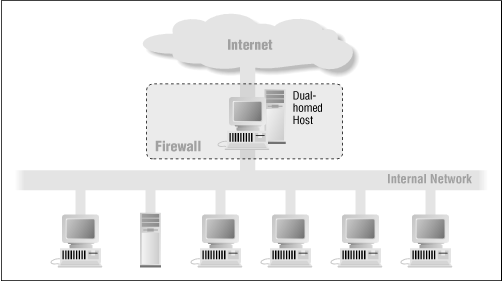
\includegraphics[width=300px]{resources/dual_homed.png}
	\caption{Arsitektur \textit{Dual-Homed}}
	\label{fig:dual_homed}
\end{figure}

\subsubsection{Arsitektur \textit{Screened Host}}

Berbeda dengan arsitektur \textit{dual-homed host} yang memberikan service dari host yang terhubung ke beberapa jaringan dengan fungsi tidak mengaktifkan fungsi routing, arsitektur \textit{screened host} memberikan layanan dari host yang hanya terhubung ke internal network dan menggunakan router terpisah seperti pada  gambar \ref{fig:screened_host}. Pada arsitektur ini, keamanan dijaga oleh packet filtering, dengan melakukan konfigurasi berikut:

\begin{enumerate}
\item Memperbolehkan \textit{internal host} untuk dapat mengakses beberapa service langsung tanpa melalui proxy.
\item Melarang semua paket dari internal host. (Untuk memaksa host itu menggunakan proxy).
\end{enumerate}

Namun pada pada arsitektur ini, jaringan internal sangat mudah diserang dari host \textit{bastion} yang berada pada internal network. Sehingga bastion host menjadi sasaran yang paling diinginkan oleh penyerang. Karena tidak ada pertahanan lagi diantara internal host dan host lain yang berada pada jaringan internal.

\begin{figure}[H]
	\centering
	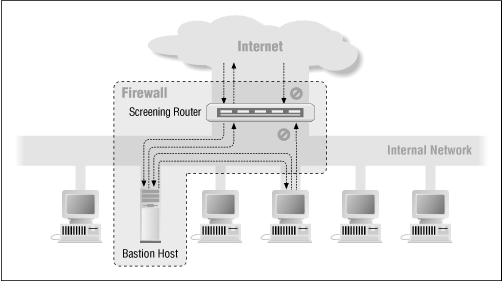
\includegraphics[width=300px]{resources/screened_host.png}
	\caption{Arsitektur \textit{Screened Host}}
	\label{fig:screened_host}
\end{figure}

\subsubsection{Arsitektur \textit{Screened Subnet}}

Arsitektur \textit{screened subnet} memiliki layer tambahan dibandingkan dengan arsitektur \textit{screened host} dengan memisahkan internal network lebih jauh dari Internet.

Arsitektur ini ditujukan agar host \textit{bastion}, yakni host yang dieskpos ke Internet, merupakan host yang paling rentan untuk diserang. Meskipun host sudah dilakukan usaha untuk melindungi host tersebut, namun host tersebut menjadi titik paling jelas untuk diserang.

\begin{figure}[H]
	\centering
	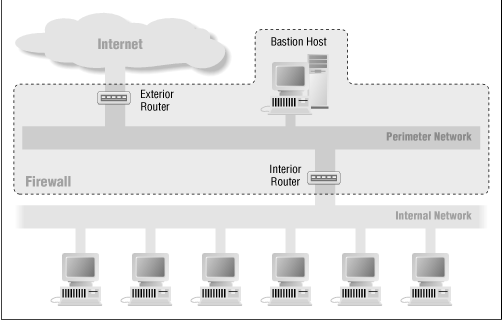
\includegraphics[width=300px]{resources/screened_subnet.png}
	\caption{Arsitektur \textit{Screened Subnet}}
	\label{fig:screened_subnet}
\end{figure}

\section{Next Generation Firewall}
Pada masa ini, firewall terbagi menjadi 2 yaitu tradisional firewall dan new generation firewall. Hal ini terjadi karena tradisional firewall tidak lagi mumpuni untuk menahan serangan yang ada di dunia internet ini. 
Tradisional firewall adalah firewall yang bekerja di \textit{network layer}(\cite{nicoll2004challenges}), menggunakan port dan protokol IP untuk mengontrol dan mencegah serangan dari jaringan.(\cite{zhong2012design}) Skema dari tradisional firewall ini dapat dilihat pada gambar berikut.
\begin{figure}[H]
	\centering
	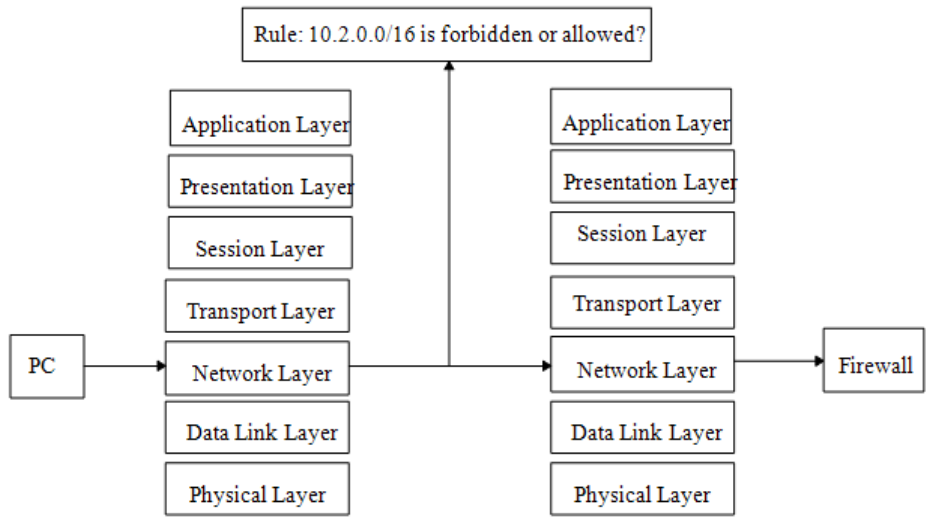
\includegraphics[width=0.8\textwidth]{resources/tradisional_firewall.png}
	\caption{Skema tradisional firewall(\cite{zhong2012design})}
	\label{fig:tradisional_firewall}
\end{figure}

Firewall ini hanya mengecek header paket sesuai dengan portnya, sehingga tidak dapat mengontrol aplikasi. Tradisional firewall yang memakai \textit{deep packet inspection} (DPI) untuk menambah keamanan juga tidak terlalu berhasil, karena memunculkan limitasi dan masalah baru. Menurut (\cite{miller2011next}), masalah tersebut adalah
\begin{itemize}
	\item Aplikasi yang tidak seharusnya berada di jaringan diperbolehkan masuk ke jaringan.
	\item Tidak semua paket yang harus diperiksa terperiksa
	\item Policy management menjadi rumit dan berbelit
	\item Performansi yang tidak memadai 
\end{itemize}

Sementara itu, Next Generation Firewall (NGFW) merupakan pengembangan dari first-generation firewall yang memiliki Deep Packet Inspection (DPI). Secara fungsionalitas NGFW merupakan gabungan dari IPS dan first-generation firewall. NGFW dapat dipandang sebagai IPS karena NGFW memiliki awareness terhadap application level payload. Hasil pengecekan kemudian digunakan untuk memutuskan apakah paket di-forward atau di-drop. (Pescatore, 2009). New Generation Firewall adalah firewall yang berjalan diatas layer aplikasi, untuk mendeteksi apakah paket tersebut sesuai dengan user`s rule atau tidak(\cite{zhong2012design}). Skema dari new generation firewall adalah sebagai berikut.
\begin{figure}[H]
	\centering
	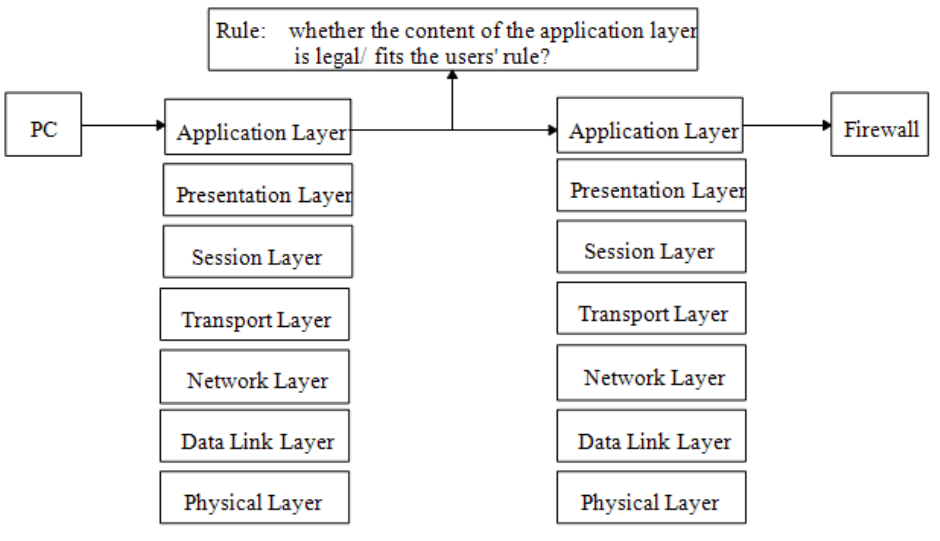
\includegraphics[width=\textwidth]{resources/NGFW.png}
	\caption{Skema new generation firewall(\cite{zhong2012design})}
	\label{fig:new_generation_firewall}
\end{figure}

Fungsi dan kemampuan utama yang dibutuhkan oleh new generation firewall adalah:
\begin{itemize}
	\item Identifikasi aplikasi (port, protocol, evasive techniques, atau SSL encryption) sebelum melakukan hal apapun
	\item Menyediakan policy-based control yang lebih jelas dan granular
	\item Secara akurat mengidentifikasi pengguna dan menggunakan informasi tersebut sebagai atribut dari policy control
	\item Menyediakan proteksi secara real-time terhadap ancaman dari jaringan, termasuk yang beroperasi pada layer aplikasi.
	\item Terintegrasi untuk meningkatkan kapasitas pencegahan ancaman
\end{itemize}

\subsection{Teknik Identifikasi aplikasi}
Teknik Identifikasi aplikasi yang digunakan oleh new generation firewall adalah
\begin{itemize}
	\item Deteksi dan dekripsi aplikasi protokol\\
	Untuk mendeteksi protokol aplikasi sehingga dapat dianalisis lebih lanjut
	\item Decode aplikasi protokol\\
	Untuk mendeteksi apakah ada aplikasi lain yang berjalan melalui protokol tersebut (tunnel), seperti Yahoo! Instant Messenger yang mungkin berada di dalam protokol HTTP
	\item Application signatures\\
	Untuk mengecek apakah aplikasi tersebut menggunakan port dan protokol yang sesuai dengan fungsinya.
	\item Heuristics
\end{itemize}

\subsection{User identification}
Teknologi ini mengidentifikasi user sehingga dapat digunakan untuk:
\begin{itemize}
	\item Mendapatkan visibilitas tentang siapa yang bertanggung jawab untuk semua aplikasi, konten, dan ancaman lalu lintas data pada jaringan tersebut
	\item Mengizinkan penggunaan identitas sebagai variabel dalam access control policies.
	\item Memfasilitasi troubleshooting/incident response
\end{itemize}

\subsection{Content identification}
Teknologi ini membuat next generation firewall dapat mencegah ancaman secara real-time, mengontrol web surfing activities, dan memfilter file atau data. Komponen dari teknologi ini adalah:
\begin{itemize}
	\item Pencegahan ancaman\\
	Komponen ini berfungsi untuk mencegah spyware, virus, dan ancaman lainnya dari jaringan. Komponen ini dibantu oleh application decoder, stream-based virus detection, spyware scanning, uniform threat signature format, dan IPS.
	\item URL filtering\\
	Komponen ini memfilter konten melalui URL.
	\item Filter file dan data\\
	Komponen ini menggunakan kelebihan dari in-depth application inspection untuk mengurangi pengiriman file dan data yang tidak terotorisasi. 
\end{itemize}

\subsection{Perbedaan performansi antara tradisional firewall dan new generation firewall}
Pada tradisional firewall, fungsi-fungsi keamanan dilakukan secara terpisah satu sama lain, seperti yang digambarkan pada gambar \ref{fig:architecture_tradisional_firewall}. Hal ini menyebabkan penggunaan system resource yang berlebihan dan tidak efisien.
\begin{figure}[H]
	\centering
	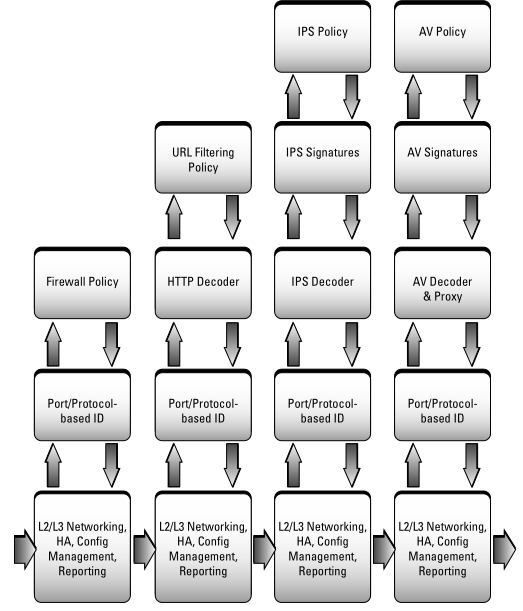
\includegraphics[width=8cm]{resources/architecture_tradisional_firewall.png}
	\caption{arsitektur proses tradisional firewall(\cite{miller2011next})}
	\label{fig:architecture_tradisional_firewall}
\end{figure}

Sebaliknya, new generation firewall menggunakan single-pass architecture untuk mengeliminasi pengecekan paket secara repetitif, mengurangi beban pada hardware dan meminimalkan latency, seperti yang dapat dilihat pada gambar berikut.

\begin{figure}[H]
	\centering
	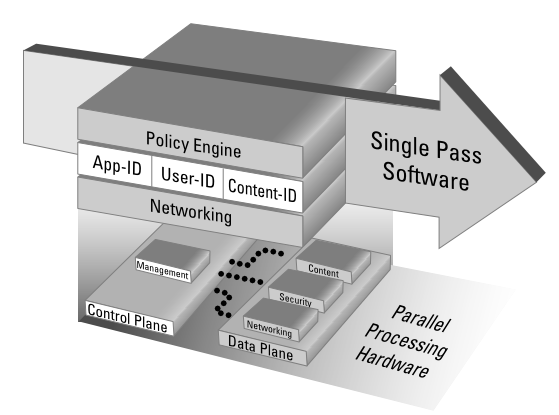
\includegraphics[width=0.7\textwidth]{resources/architecture_NGFW.png}
	\caption{arsitektur proses new generation firewall(\cite{miller2011next})}
	\label{fig:architecture_NGFW}
\end{figure}

\section{Deep Packet Inspection}
Deep Packet Inspection (DPI) adalah salah satu teknologi utama untuk mengidentifikasi dan mengotentikasi protokol dan aplikasi yang dibawa bersama IP(\cite{allot2007digging}). \textit{Standard packet inspection process} hanya mengekstrak informasi dasar dari suatu protokol seperti IP address (tujuan, sumber) dan informasi koneksi low-level lainnya, yang biasanya berada pada header paket tersebut. Inspeksi ini tidak mendapatkan informasi yang cukup untuk dapat menyimpulkan apakah aplikasi tersebut aman atau tidak. 
\begin{figure}[H]
	\centering
	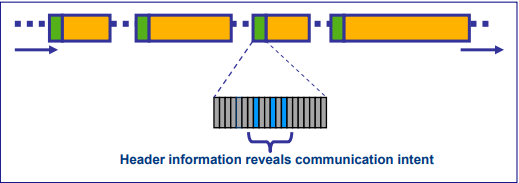
\includegraphics[width=0.8\textwidth]{resources/standard_inspection.png}
	\caption{standard packet inspection (\cite{allot2007digging})}
	\label{fig:standard_inspection}
\end{figure}
Sebaliknya, DPI menyediakan informasi tentang aplikasi tersebut. Hal ini dicapai dengan menganalisis konten pada header paket dan payload paket pada suatu transaksi paket. Oleh karena itu, DPI dapat menyediakan kemampuan untuk menganalisa penggunaan jaringan dan mengoptimasi performansi jaringan. 

Komponen yang digunakan untuk memberi identitas pada aplikasi dan protokol disebut signature. Signature ini dapat juga diumpamakan seperti fingerprint pada manusia, dimana tidak ada yang sama satu dengan yang lainnya. Oleh karena itu, signature digunakan untuk mengidentifikasi aplikasi dan protokol. Signature pada aplikasi harus dicek secara berkala, karena signature tersebut dapat berubah seiring aplikasi update atau revisi protokol.

Walaupun signature tersebut dikembangkan dengan tujuan keunikan dan untuk mengidentifikasi suatu aplikasi atau protokol, ada kalanya signature tersebut tidak robust. Terdapat istilah \textit{false positives} dan \textit{false negatives} karena signature tersebut. \textit{False positives} merujuk pada keadaan salah mengelompokkan atau salah mengidentifikasi, seperti suatu aplikasi diidentifikasi sebagai sesuatu, namun sebenarnya bukan. \textit{False negatives} merujuk pada keadaan dimana suatu aplikasi atau protokol tidak teridentifikasi secara konsisten sebagai sesuatu yang sama. Contohnya, beberapa aplikasi akan berperilaku berbeda apabila koneksi yang dilakukan melalui proxy atau tidak. Salah satu cara untuk membuat signature tersebut menjadi lebih robust adalah dengan menggunakan beberapa pola kombinasi.

\subsection{Metode analisis signature}
Ada beberapa metode analisis yang digunakan untuk mengidentifikasi dan mengelompokkan paket, yaitu:
\begin{itemize}
	\item Analisis berdasarkan port\\
	Analisis ini merupakan analisis yang paling mudah dan paling dikenal. Namun analisis ini tidak cukup untuk mengidentifikasi aplikasi sendirian, dikarenakan sudah banyak aplikasi yang memakai random port atau menyamar sebagai aplikasi lain pada port tertentu.
	\item Analisis berdasarkan string match\\
	Analisis ini akan mencari suatu string pada konten paket tersebut. Hal ini dilakukan karena banyak aplikasi yang menyertakan nama aplikasi tersebut pada protokolnya. 
	\item Analisis berdasarkan numerical properties\\
	Analisis ini melibatkan perhitungan dan karakteristik numerik pada paket tersebut, seperti payload length, banyaknya paket yang dikirim untuk respon transaksi tertentu, dan numerical offset dari suatu string dalam paket tersebut. Analisis ini juga tidak cukup berdiri sendiri untuk mengidentifikasi aplikasi.
	\item Analisis berdasarkan perilaku dan heuristics\\
	Analisis ini merujuk pada bagaimana biasanya protokol berperilaku dan beroperasi. Analisis heuristik pada umumnya berasal dari hasil statistik dari paket yang diamati.
\end{itemize}

\section{Malware}
\textit{Malicious software} menurut (\cite{idika2007survey}) memiliki banyak baentuk salah satunya adalah Malicious Code (MC). Menurut (\cite{attackingmalcode}), malicious code merupakan kode yang ditambahkan, diubah, atau dihilangkan dari sistem software untuk membahayakan atau mengubah fungsi yang diharapkan dapat dilakukan oleh sistem.

Virus merupakan program komputer yang mereplikasi dengan menyisipkan dirinya ke program lain. Program yang disisipi oleh virus menjadi terinfeksi disebut inang. Hal ini yang membedakan virus dengan malware lain, untuk melakukan fungsinya virus memerlukan inang (\cite{attackingmalcode}).

Worm merupakan program komputer yang mereplikasi dirinya dengan menjalankan kode worm yang manjadi sebuah program tersendiri. Bagian yang membedakan worm dan virus, worm tidak memerlukan inang untuk melakukan fungsinya. Selain itu, virus dan worm juga berbeda pada cara penyebarannya. Pada umumnya, virus berusaha untuk menyebar melalui file atau program pada satu komputer. Sedangkan worm berusaha untuk menginfeksi sebanyak mungkin komputer melalui jaringan (\cite{attackingmalcode}).

Trojan horse merupakan malicious code yang tambahkan oleh desainer dalam sebuah aplikasi atau sistem. Aplikasi tersebut menjalankan fungsinya, namun melakukan aktifitas malicious seperti merekam kegiatan pengguna dan mengirimkannya ke pembuatnya. Trojan horse pada umumnya berkaitan dengan mengakses dan mengirimkan informasi tanpa otorisasi dari pengguna. Trojan horse dapat dikategorikan sebagai spyware. 


\section{Malware Detection}

Pada (\cite{idika2007survey}) teknik untuk mendeteksi malware dibedakan menjadi dua, yakni: signature-
based dan anomaly-based. Terdapat bentuk khusus anomaly-based yakni specification-based. Setiap teknik memiliki jenis static, dynamic, dan hybrid.

\subsection{Anomaly-based Detection}

Pada (\cite{idika2007survey}) dijelaskan, anomaly-based detection memiliki dua fasa, yakni fasa training, dan fasa deteksi. Pendeteksian jenis ini memiliki kelebihan, yakni dapat mendeteksi serangan yang sebelumnya belum dikenali. Namun, deteksi jenis ini memiliki tingkat kesalahan pendeteksian yang tinggi. Anomaly based-detection melakukan pendeteksian dengan cara membuat pendekatan perilaku yang valid dilakukan oleh sebuah sistem.

\begin{figure}[H]
	\centering
	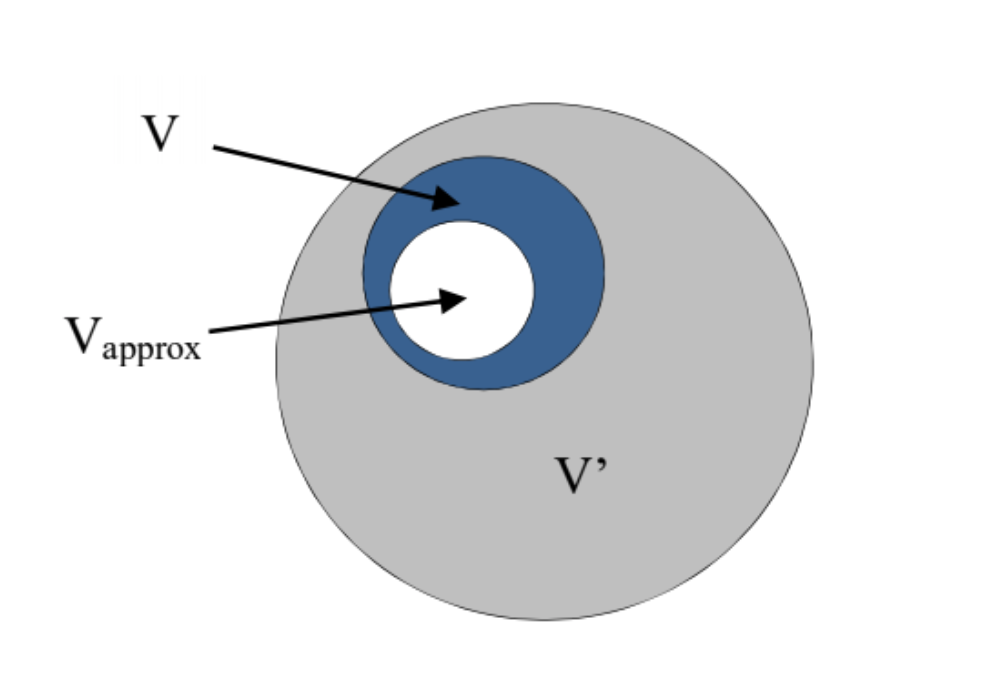
\includegraphics[width=220px]{resources/anomaly_illustration.png}
	\caption{Ilustrasi karakterisasi perilaku pada anomaly-based detection}
	\label{fig:anomaly_illust}
\end{figure}

Gambar \ref{fig:anomaly_illust} menggambarkan bagaimana anomaly-based detection mengkarakterisasi perilaku sistem. V merupakan himpunan perilaku yang tidak bertentangan dengan requirement. V’ merupakan himpunan perilaku yang yang tidak valid. Vapprox merupakan hasil pendekatan yang dilakukan oleh anomaly-based detection.

\subsection{Signature-based Detection}
Signature-based detection dalam (\cite{idika2007survey}) merupakan teknik yang menggunakan malicious-model untuk mendeteksi malware. Kumpulan dari malicious-model (signature) menjadi knowledge base dari system pendeteksi jenis ini. Sehingga pada Gambar \ref{fig:signature_illust}, diilustrasikan bahwa S (kumpulan signature) merupakan subset dari U yang merupakan seluruh signature dari perilaku malicious. Karena keterbatasan media penyimpanan, S akan sangat kecil jika dibandingkan dengan U yang sangat besar.

\begin{figure}[H]
	\centering
	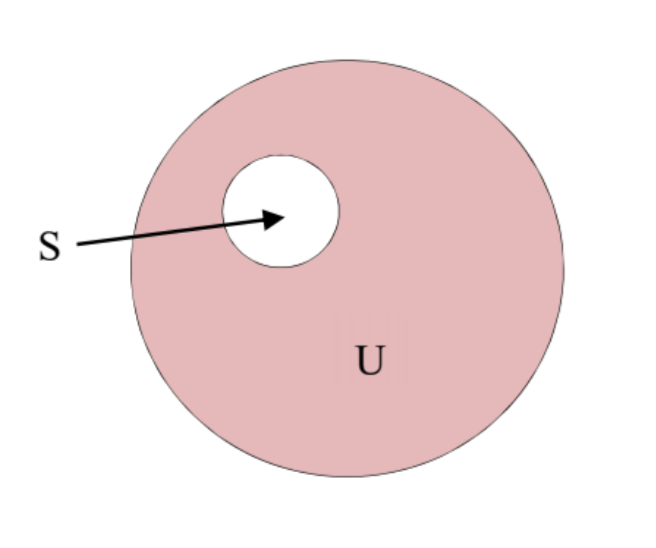
\includegraphics[width=190px]{resources/signature_illustration.png}
	\caption{Ilustrasi himpunan signature terhadap seluruh malicious signature}
	\label{fig:signature_illust}
\end{figure}

\section{Iptables}

Menurut (\cite{purdy2004linux}) Netfilter adalah bagian dari kernel Linux yang berfungsi untuk memproses paket dari jaringan. Iptables adalah perintah untuk mengatur \textit{Netfilter} yang dapat digunakan pada \textit{user-space}. Arsitektur dari iptables dikelompokkan berdasarkan fungsinya, yaitu
\begin{itemize}
	\item Filter\\
	Digunakan untuk mengatur keluar masuknya paket.
	\item \textit{Network address translation} (NAT)\\
	Digunakan dengan \textit{connection tracking} untuk melakukan Network Address Translation (NAT).
	\item Packet mangling\\
	Digunakan untuk memanipulasi paket.	
\end{itemize} 

Fungsi-fungsi tersebut memiliki \textit{chain} (urutan) pemrosesannya masing-masing. Aturan tersebut berisikan syarat (\textit{matches}) dan target. Syarat dari aturan tersebut akan menentukan paket mana saja yang akan terkena aturan tersebut, sementara target akan menentukan apa yang akan dilakukan oleh paket yang memenuhi syarat tersebut. Apabila tidak ada syarat (\textit{match criteria}) maka semua paket dianggap memenuhi syarat. Sebaliknya, apabila tidak ada target, maka paket tidak akan diproses. Syarat yang dapat digunakan antara lain adalah IP (\textit{Internet Protocol}) dan \textit{MAC addresses}.
Netfilter memiliki beberapa \textit{built-in target}, yaitu:
\begin{itemize}
	\item \textit{ACCEPT}\\
	Mengijinkan paket untuk menuju proses selanjutnya.
	\item \textit{DROP}\\
	Menghentikan proses paket sepenuhnya.
	\item \textit{QUEUE}\\
	Mengirimkan paket ke userspace.
	\item \textit{RETURN}\\
	Menghentikan proses pada user-defined chain dan melanjutkan proses ke chain sebelum user-defined chain dipanggil.
\end{itemize}
\subsection{Hooks point}
\textit{Netfilter} memiliki 5 poin didalam alur pemrosesan paket, yaitu :
\begin{itemize}
	\item \textit{PREROUTING}\\
	Poin yang akan memproses paket yang baru datang dari \textit{network interface} (setelah melalui proses pengecekan \textit{checksum}).
	\item \textit{INPUT}\\
	Poin yang akan memproses paket yang akan dilanjutkan ke proses lokal.
	\item \textit{FORWARD}\\
	Poin yang akan memproses paket yang keluar masuk melalui \textit{gateway} komputer.
	\item \textit{POSTROUTING}\\
	Poin yang akan memproses paket yang akan meninggalkan \textit{network interface}.
	\item \textit{OUTPUT}\\
	Poin yang akan memproses paket yang baru saja melewati proses lokal.
\end{itemize}
aturan dasar (\textit{built-in chain}), dan dapat ditambahkan aturan lain yang diinginkan.

\subsection{Alur pemrosesan paket}
Fungsi-fungsi dari arsitektur iptables tersebut disebut juga \textit{tables}, dan fungsi-fungsi tersebut memiliki alur pemrosesan dasar sebagai berikut.\\
\begin{figure}[H]
	\centering
	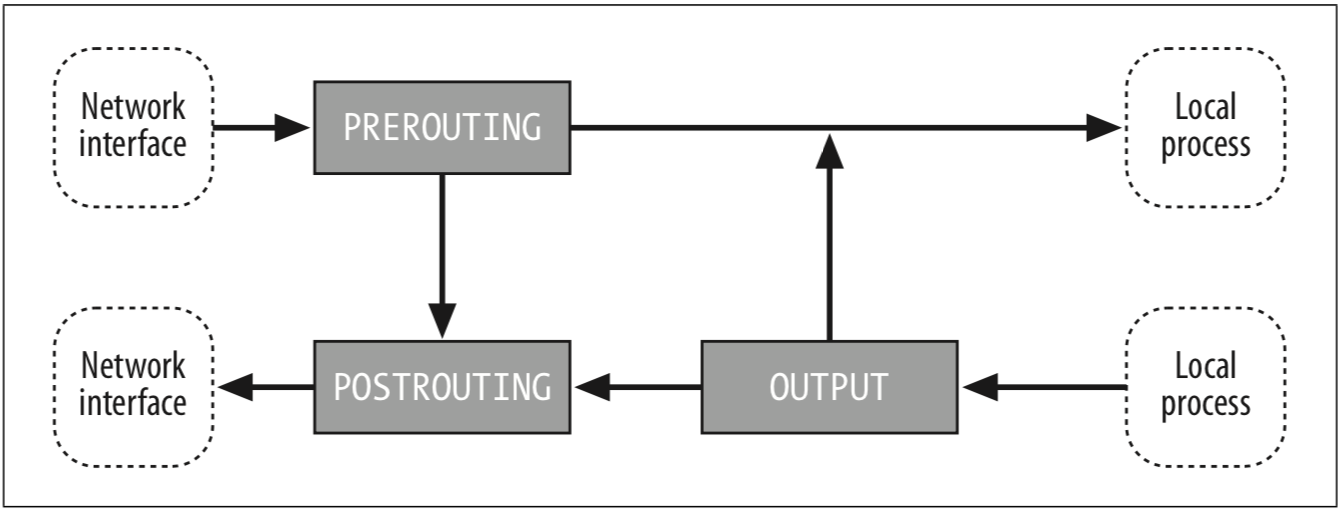
\includegraphics[width=\textwidth]{resources/nat_table.png}
	\caption{Alur pemrosesan paket dan \textit{hook} yang digunakan pada tabel \textit{NAT}.}
	\label{fig:packetflow_NAT}
\end{figure}

\begin{figure}[H]
	\centering
	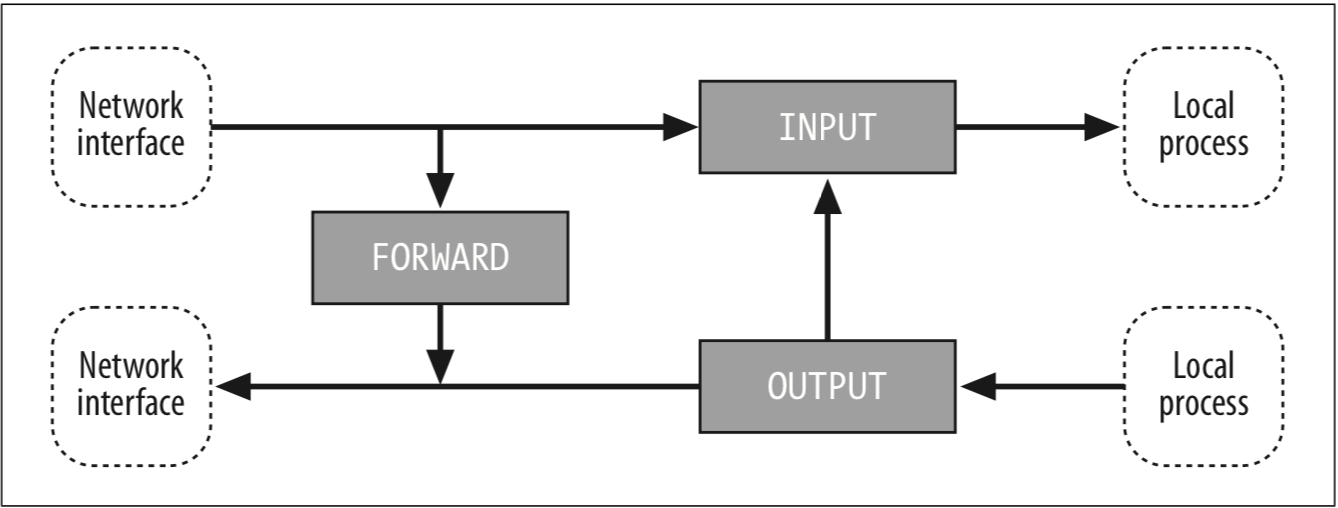
\includegraphics[width=\textwidth]{resources/filter_table.png}
	\caption{Alur pemrosesan paket dan \textit{hook} yang digunakan pada tabel \textit{filter}.}
	\label{fig:packetflow_filter}
\end{figure}

\begin{figure}[H]
	\centering
	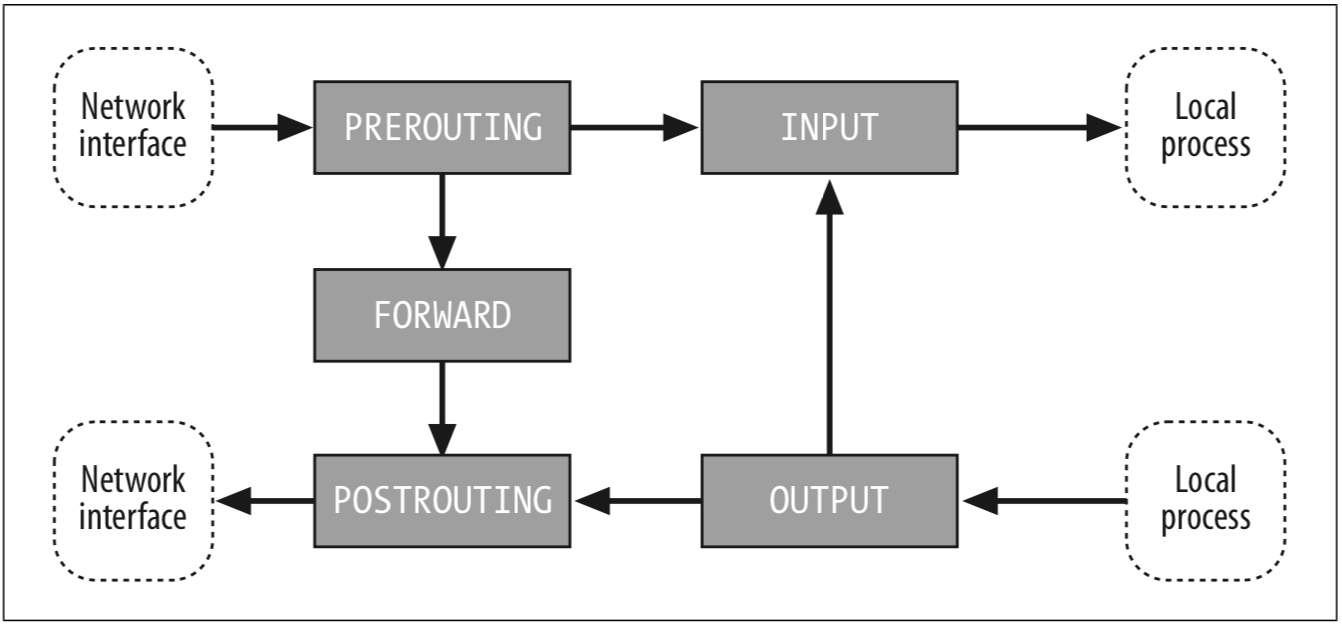
\includegraphics[width=\textwidth]{resources/mangling_table.png}
	\caption{Alur pemrosesan paket dan \textit{hook} yang digunakan pada tabel \textit{mangling}.}
	\label{fig:packetflow_mangling}
\end{figure}

Paket yang melewati \textit{chain} akan terkena aturan sesuai dengan urutannya. Apabila paket tersebut tidak sesuai kriteria, maka paket akan bergerak ke aturan selanjutnya. Jika paket tersebut tidak memenuhi kriteria sampai aturan yang paling akhir, maka paket tersebut akan diperlakukan sesuai dengan \textit{chain\textquotesingle s policy}. 
Berdasarkan Gambar , urutan alur paket yang melewati \textit{tables} dan \textit{chains} dapat dilihat pada tabel-tabel berikut.

\begin{table}[H]
	\caption{Alur paket yang melewati network interface ke network interface lainnya (forwarding)}
	\label{table:network_to_network}
	\centering
	\begin{tabular}{ll}
		\hline
		\rowcolor[HTML]{C0C0C0} 
		table  & chain       \\ \hline
		mangle & PREROUTING  \\
		nat    & PREROUTING  \\
		mangle & FORWARD     \\
		filter & FORWARD     \\
		mangle & POSTROUTING \\
		nat    & POSTROUTING \\ \hline
	\end{tabular}
\end{table}

\begin{table}[H]
	\caption{Alur paket yang melewati network interface ke proses lokal (input)}
	\label{table:network_to_local}
	\centering
	\begin{tabular}{ll}
		\hline
		\rowcolor[HTML]{C0C0C0} 
		table  & chain      \\ \hline
		mangle & PREROUTING \\
		nat    & PREROUTING \\
		mangle & INPUT      \\
		filter & INPUT      \\ \hline
	\end{tabular}	
\end{table}

\begin{table}[H]
	\caption{Alur paket yang datang dari proses lokal ke network interface (output)}
	\label{table:local_to_network}
	\centering
	\begin{tabular}{ll}
		\hline
		\rowcolor[HTML]{C0C0C0} 
		table  & chain       \\ \hline
		mangle & OUTPUT      \\
		nat    & OUTPUT      \\
		filter & OUTPUT      \\
		mangle & POSTROUTING \\
		nat    & POSTROUTING \\ \hline
	\end{tabular}
\end{table}

\begin{table}[H]
	\caption{Alur paket yang datang dari proses lokal ke proses lokal lainnya (local)}
	\label{table:local_to_local}
	\centering
	\begin{tabular}{ll}
		\hline
		\rowcolor[HTML]{C0C0C0} 
		table  & chain  \\ \hline
		mangle & OUTPUT \\
		nat    & OUTPUT \\
		filter & OUTPUT \\
		filter & INPUT  \\
		mangle & INPUT  \\ \hline
	\end{tabular}
\end{table}

\chapter{Analisis dan Perancangan}

\section{Analisis Malware WannaCry}

Pada bagian ini, peneliti memfokuskan analisa malware WannaCry pada analisa lalu lintas paket yang dilakukan oleh host terinfeksi dengan melakukan machine-in-the-middle. Analisis malware WannaCry dilakukan dengan melakukan \textit{sniffing} dengan menggunakan 3 host dengan jaringan terisolasi seperti pada gambar \ref{fig:analisis_malware_net}. 
Ketiga host tersebut memiliki arsitektur yang sama yakni x86\_64 sehingga tidak ada alignment (seperti little endian dan big endian) berbeda.

\begin{figure}[H]
	\centering
	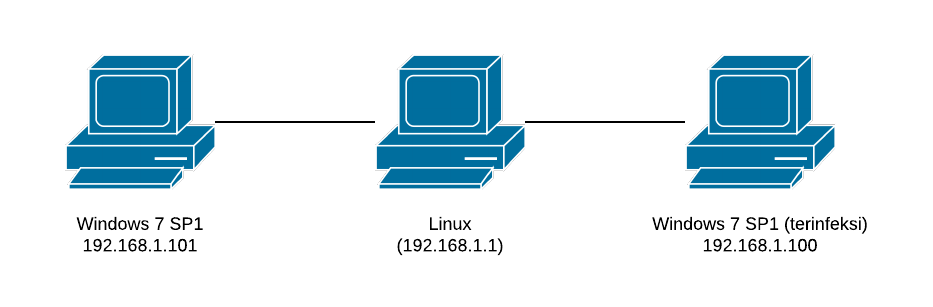
\includegraphics[width=400px]{resources/analisis_malware_net.png}
	\caption{Susunan jaringan untuk analisis malware WannaCry}
	\label{fig:analisis_malware_net}
\end{figure}

Host linux (192.168.1.1) menjadi host dengan dua interface yang dijadikan \textit{bridge}. Sehingga host Windows 7 terinfeksi (192.168.1.100) dapat berkomunikasi dengan host Windows 7 SP1 (192.168.1.101) hanya melalui 192.168.1.1. Kemudian pada host linux dilakukan sniffing dengan menggunakan tcpdump. dengan command sebagai berikut:

\begin{verbatim}
$ tcpdump -s0 -i br0 -vv -w output.wannacry-1.pcap
\end{verbatim}

\section{Karakteristik Malware WannaCry}

Dari pengelompokan malware menjadi worm, virus dan trojan horse menurut (\cite{idika2007survey}) maka WannaCry digolongkan sebagai worm. Sesuai dengan karakteristik yang disebutkan WannaCry memiliki kapabilitas menginfeksi melalui network. WannaCry memiliki dua buah bagian utama: ransomware, dan worm penginfeksi, yang melakukan penyebaran melalui protokol SMB. Jika sebuah host hanya menjalankan bagian ransomware saja, maka tidak akan ada penyebaran yang dilakukan, seperti ditunjukan pada Gambar \ref{fig:no_infect_action}.

Sedangkan jika host menjalankan bagian dropper, dropper tersebut akan menjalankan worm penginfeksi dan sekaligus menjalankan ransomware. Pada Gambar \ref{fig:infect_action} terlihat host 192.168.1.100  mencoba melakukan koneksi ke port \verb|445/tcp| setiap host yang berada pada subnet yang sama.

\begin{figure}[H]
	\centering
	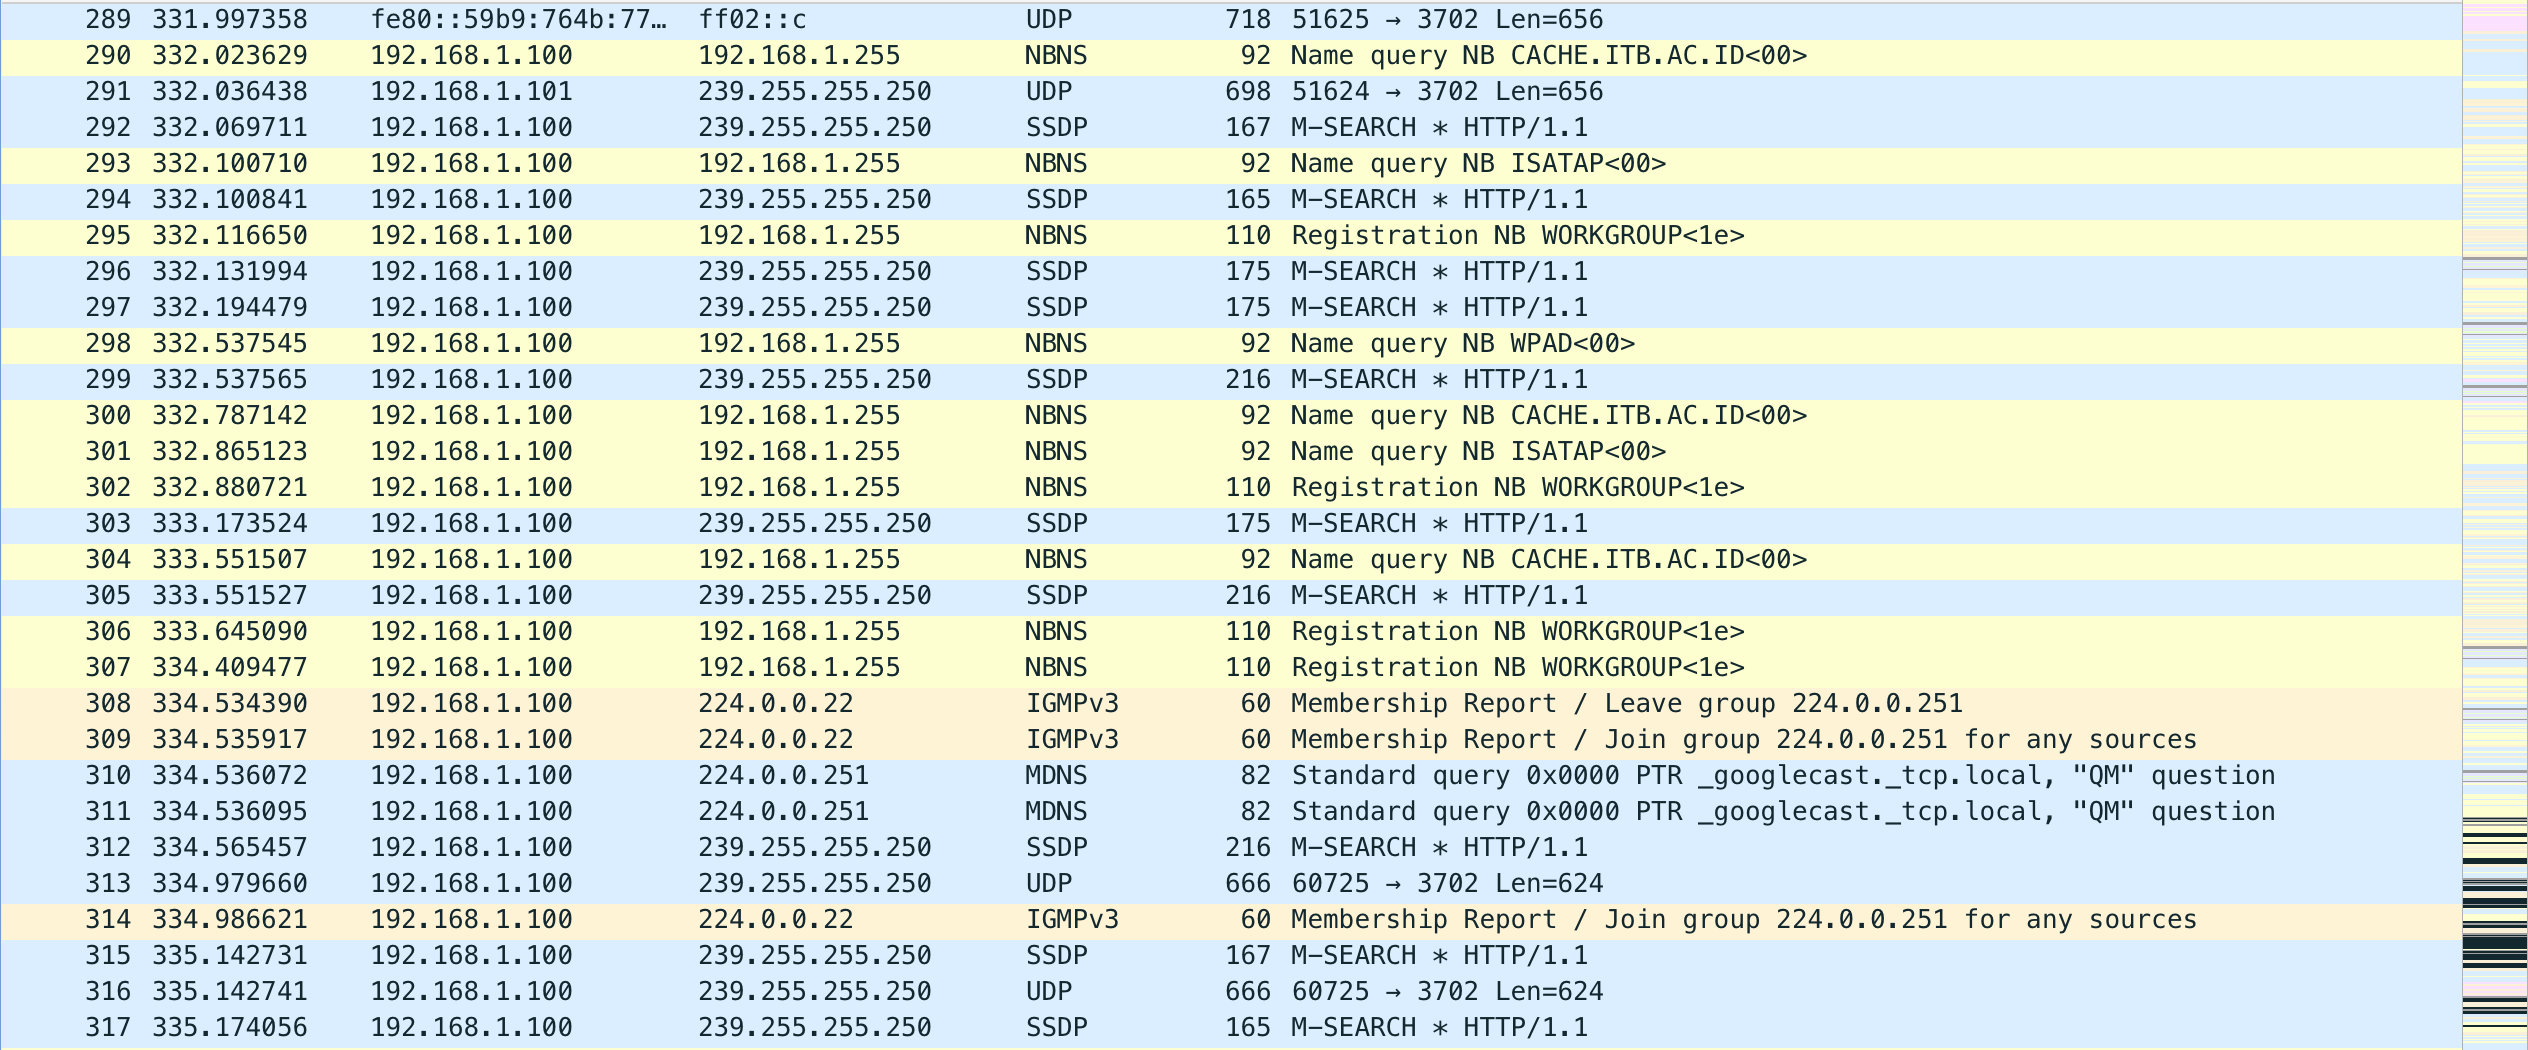
\includegraphics[width=\textwidth]{resources/no_infect_action.png}
	\caption{Paket pada host terinfeksi ransomware tanpa worm penginfeksi}
	\label{fig:no_infect_action}
\end{figure}

\begin{figure}[H]
	\centering
	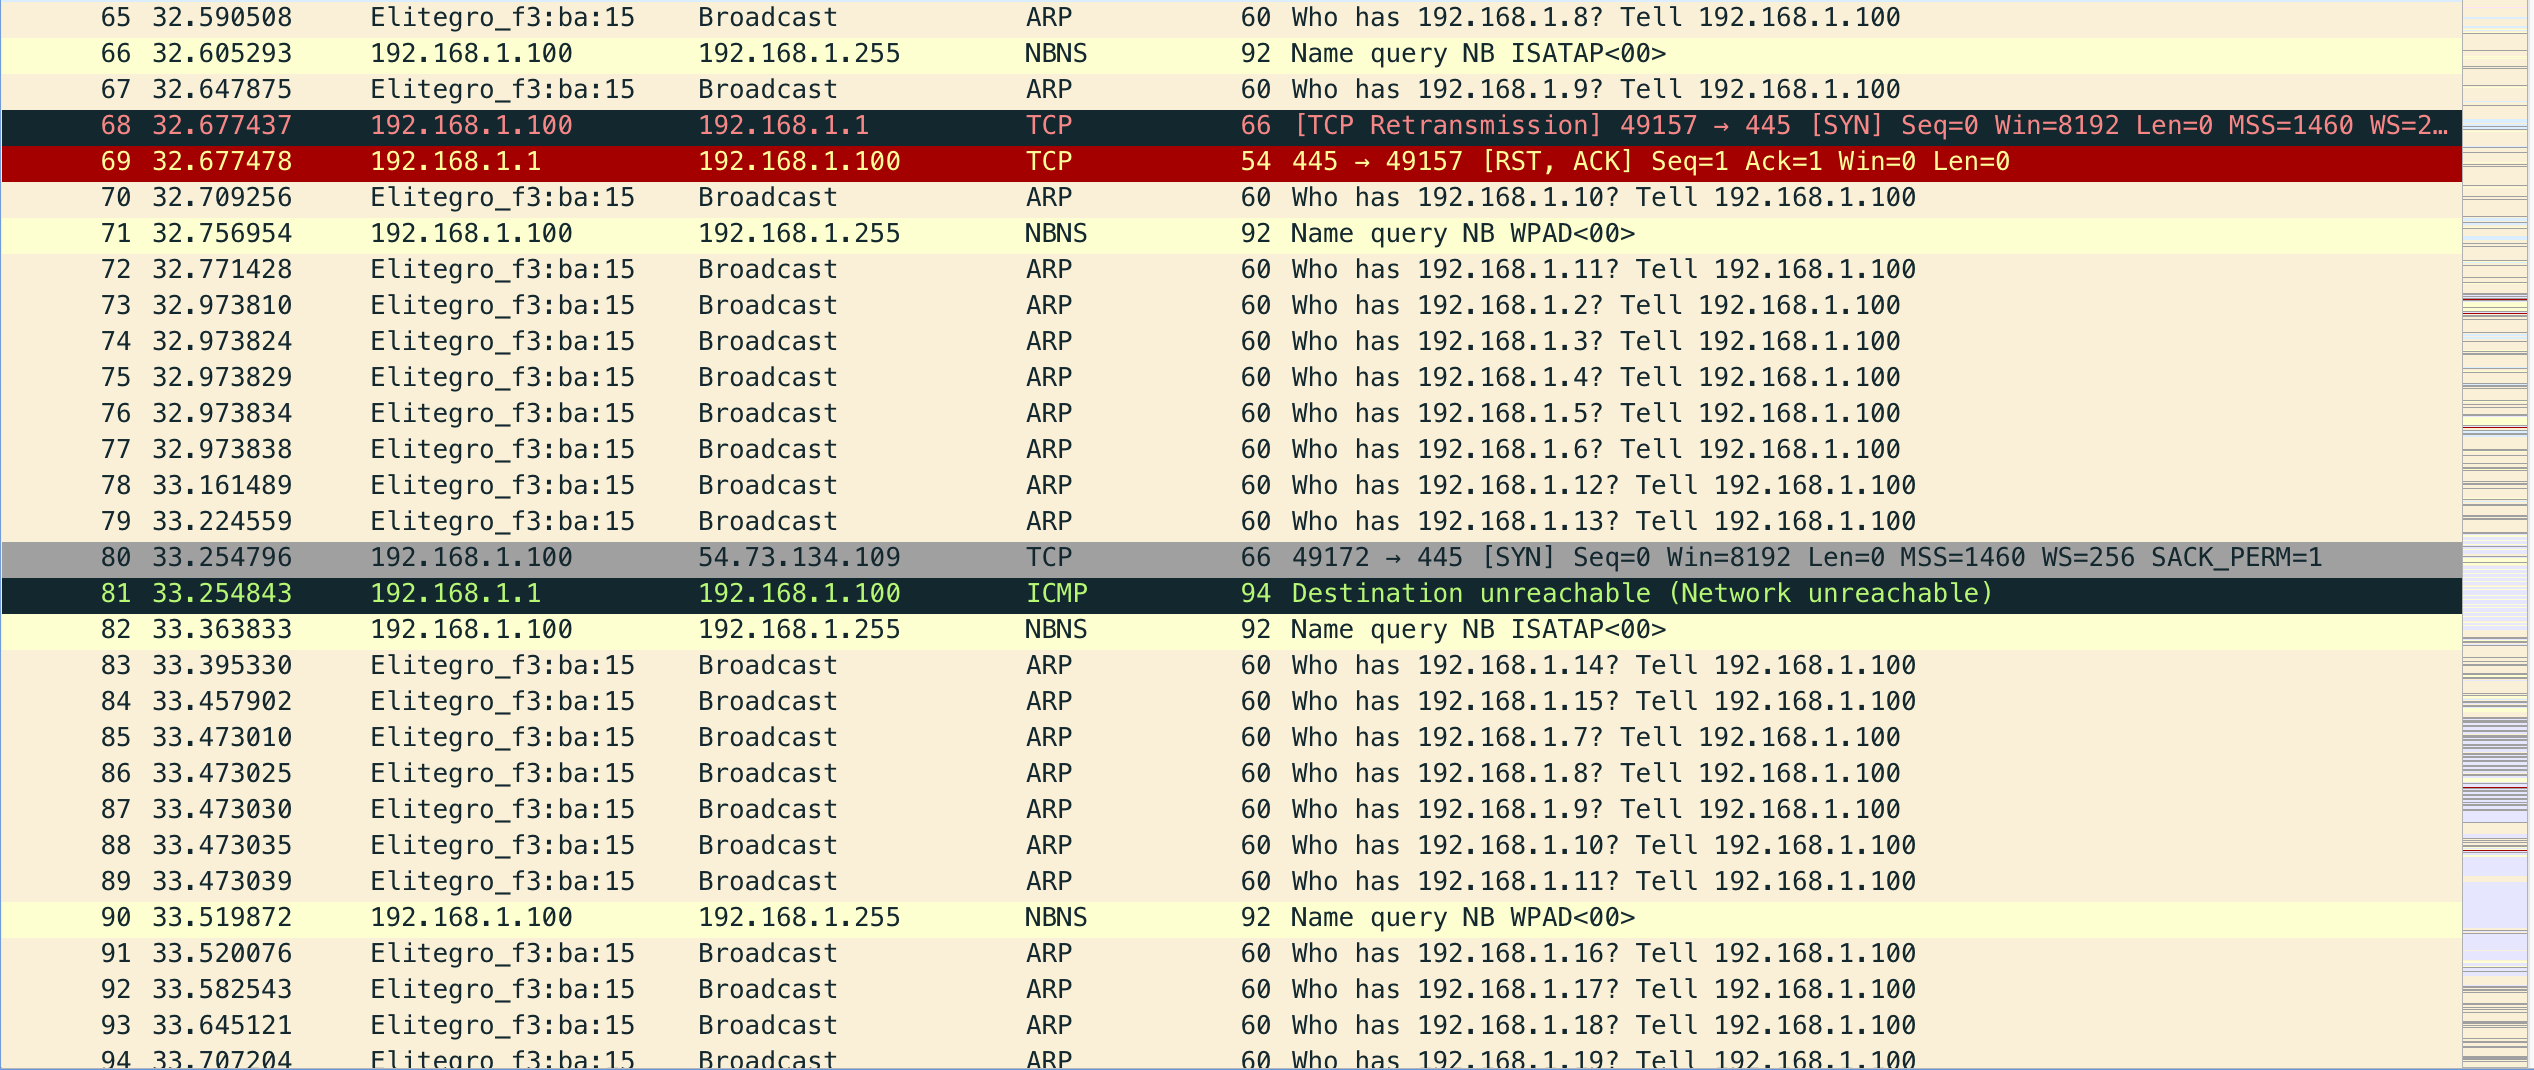
\includegraphics[width=\textwidth]{resources/infect_action.png}
	\caption{Paket pada host terinfeksi ransomware dengan dropper}
	\label{fig:infect_action}
\end{figure}

Ransomware merupakan kategori malicious software yang ketika dijalankan akan menonaktifkan fungsi tertentu dari komputer dengan sebuah cara. Kemudian ransomware akan menampilkan pesan untuk meminta pembayaran untuk mengembalikan fungsi yang dinonatifkan. Sehingga malware seakan-akan melakukan penyandraan terhadap komputer. (\cite{o2012ransomware}).

\section{Analisis Payload SMB oleh WannaCry}

Dari riset yang telah dilakukan oleh \cite{islam2018smb}, WannaCry melakukan exploit terhadap vulnerability yang menurut EternalBlue dan DoublePulsar yang ada pada implementasi SMB1.

\subsection{Vulnerability EternalBlue}
EternalBlue merupakan vulnerability yang diakibatkan oleh 3 buah bug (\cite{islam2018smb}) dan (\cite{grossman2017check}) yakni:
\begin{enumerate}
	\item Wrong casting bug
	\item Wrong parsing function bug
	\item Non-paged pool allocation bug
\end{enumerate}

Pada host 192.168.1.100 paket yang dikirimkan malware untuk mengeksploitasi vulnerability seperti yang disebutkan (\cite{islam2018smb}), yakni dengan mengirimkan \verb|SMB_COM_NT_TRANSACT| terlihat pada Gambar \ref{fig:trans_nop}, diikuti dengan \verb|SMB_COM_TRANSACTION2_SECONDARY| seperti pada Gambar \ref{fig:trans2_secondary}.

\begin{figure}[H]
	\centering
	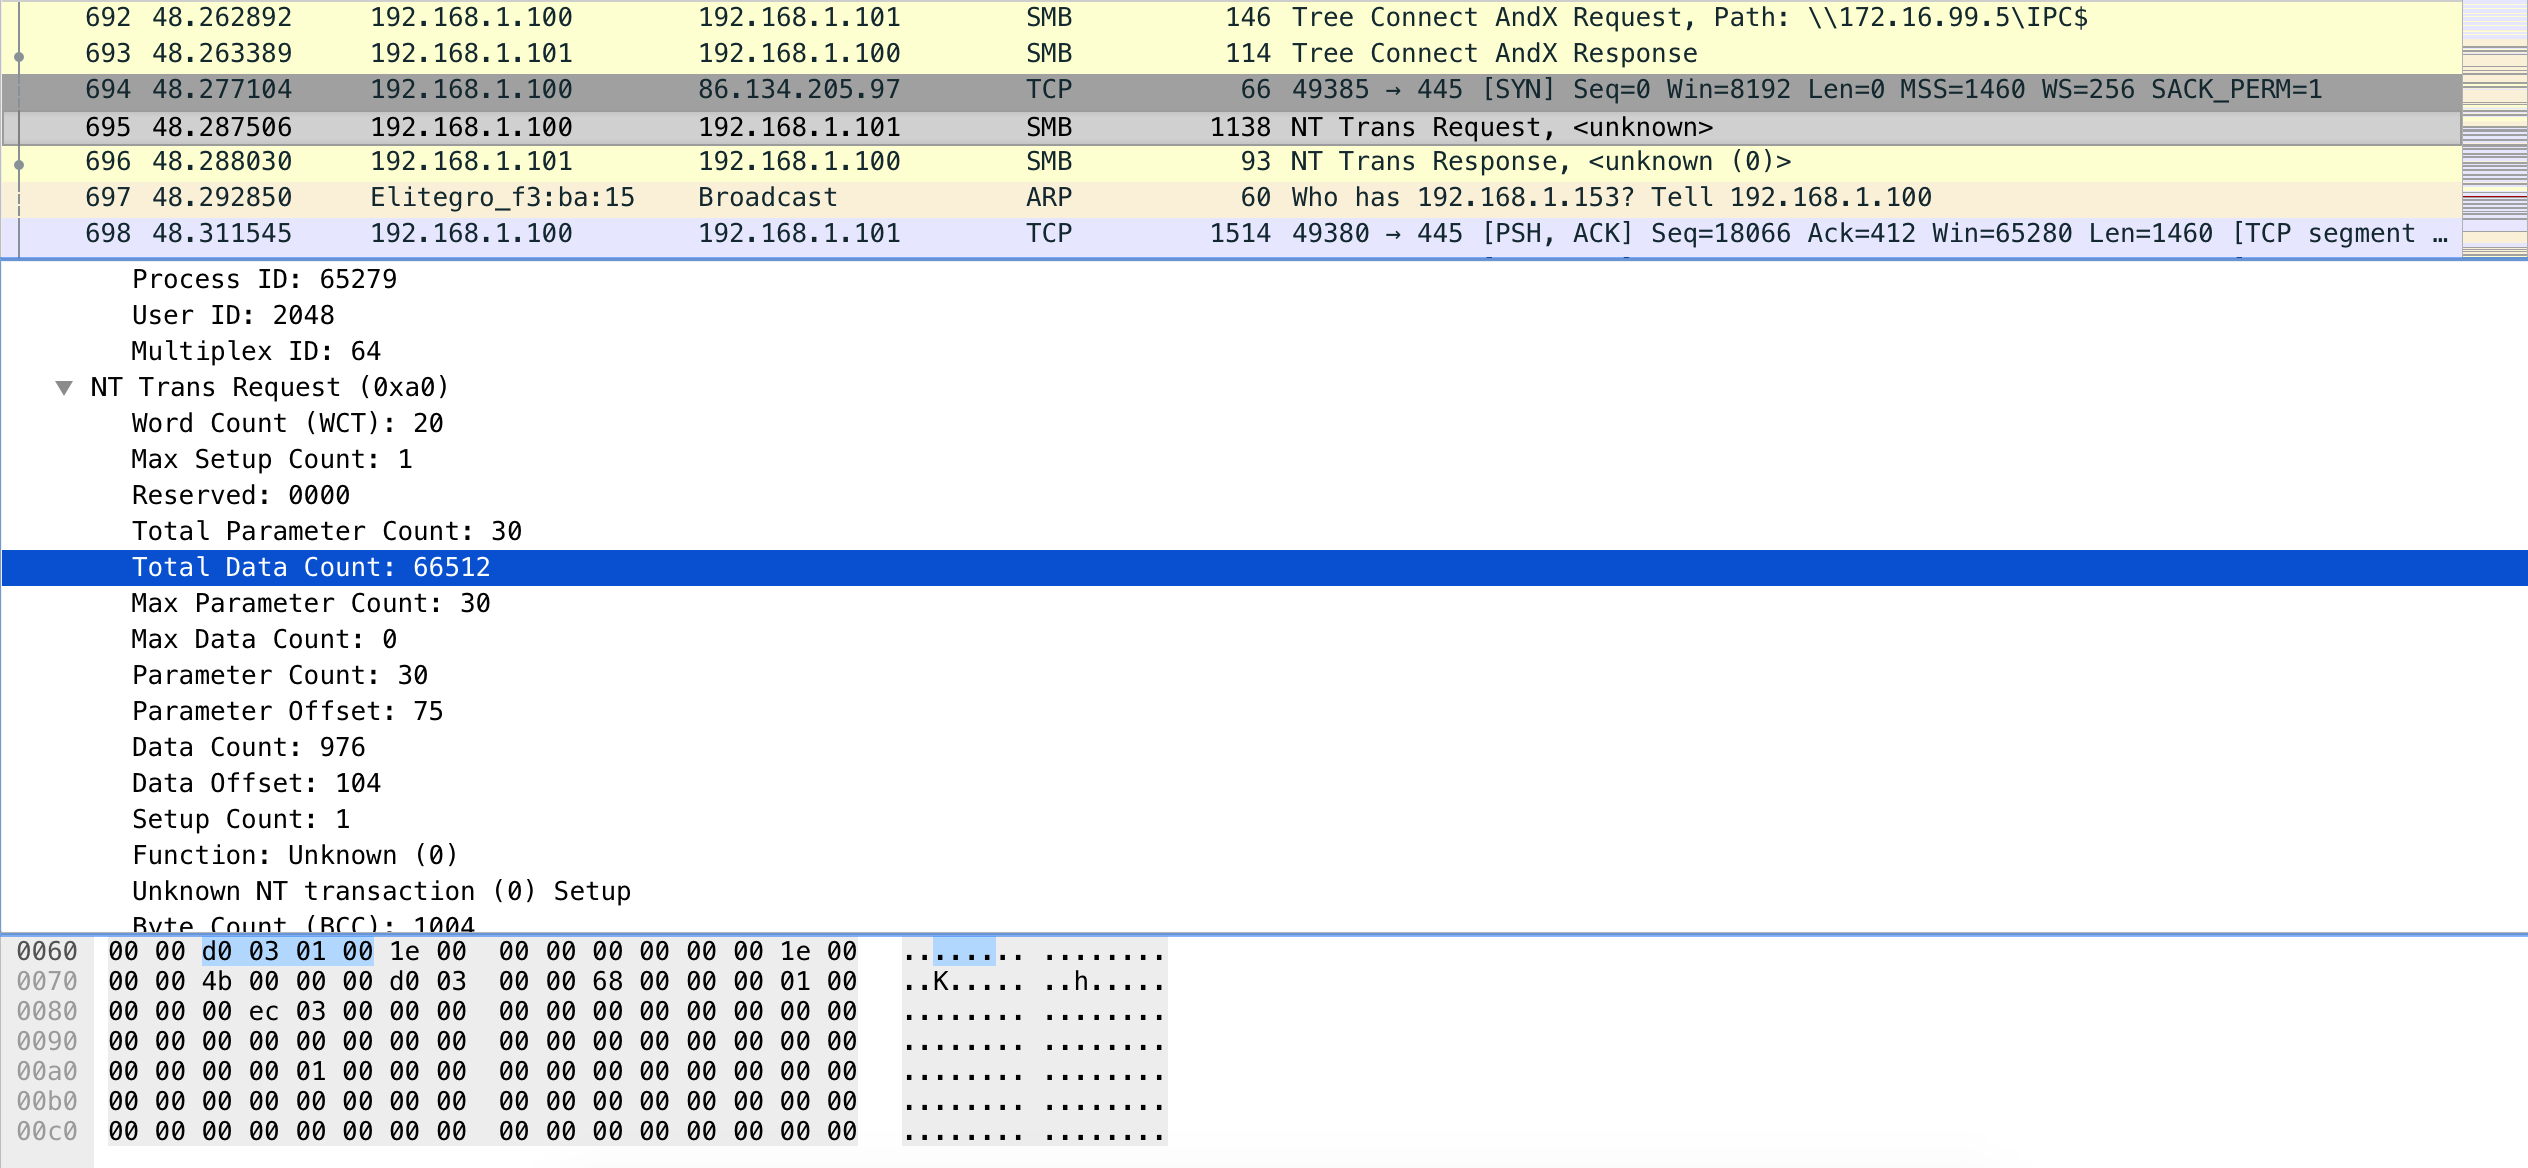
\includegraphics[width=\textwidth]{resources/trans_nop.png}
	\caption{Paket SMB\_COM\_NT\_TRANSACT dari host terinfeksi}
	\label{fig:trans_nop}
\end{figure}
\begin{figure}[H]
	\centering
	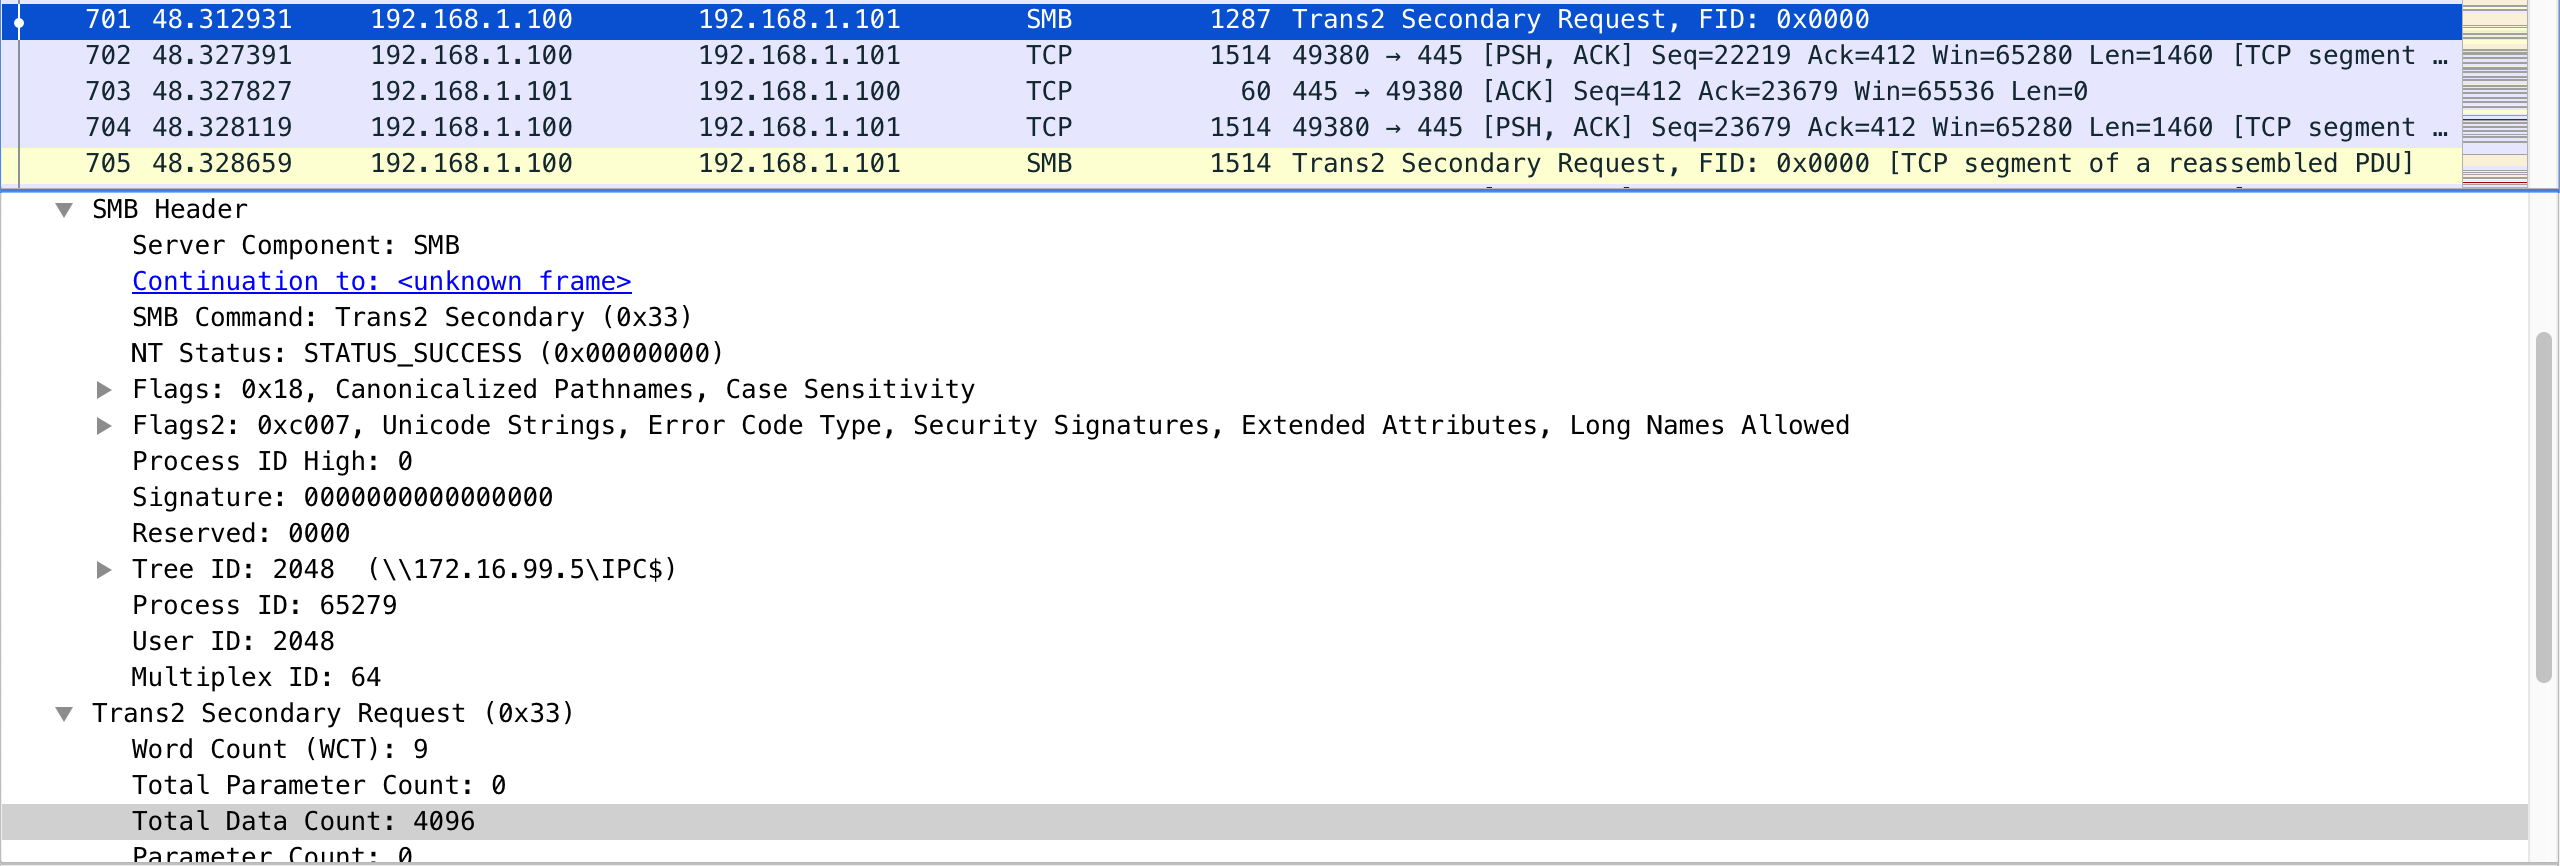
\includegraphics[width=\textwidth]{resources/trans2_secondary.png}
	\caption{Paket SMB\_COM\_TRANSACTION2\_SECONDARY dari host terinfeksi}
	\label{fig:trans2_secondary}
\end{figure}

\subsection{Vulnerability DoublePulsar}


Pada malware wannacry

\section{Deteksi Protokol}
Untuk membuat sebuah firewall yang dapat melakukan block terhadap payload malicious yang dikirim oleh WannaCry, firewall harus dapat membedakan jenis paket. Penentuan jenis paket ini dapat dilakukan dengan melakukan inspeksi paket yang merupakan fitur dari DPI (Deep Packet Inspection).

\subsection{OpenDPI}
Menurut (\cite{khalife2013performance}), OpenDPI merupakan salah satu kakas yang merupakan turunan dari produk PACE dari Ipoque. OpenDPI pada awalnya dikembangkan untuk melakukan deteksi dan mengatur lalu lintas data peer-to-peer dengan melakukan inspeksi paket. OpenDPI pada intinya merupakan library yang didesain untuk melakukan klasifikasi pada lalu lintas data berdasarkan protokol aplikasi yang digunakan.

\subsection{nDPI}

Menurut (\cite{deri2014ndpi}), nDPI merupakan superset dari 


* The OpenDPI library is written in C and it is divided in two main components: the core library (responsible for handling raw packets, decoding IP layers 3 and 4, and extracting basic information such as IP address and port) and plugin dissectors (responsible for detecting the ~100 protocols supported by OpenDPI). nDPI inherited this two-layer architecture but it addressed several issues present in the OpenDPI design: 

* The OpenDPI library was designed to be extensible, but in practice the data structures used internally were static. For instance, many data-types and bitmaps, used to keep the state for all supported protocols, were bound to specific sizes (e.g., 128 bits) and thus limiting the number of identifiable protocols. 

* Whenever a protocol was detected, the library tried to find further protocol matches instead of just returning the first match. The result was a performance penalty without a real need of requiring extra detection work. 

* No encrypted protocol support (e.g., HTTPS). While encryption is designed to preserve privacy and regular DPI libraries are not expected to decode the some information can be gleaned to suggest the nature of the information carried on a specific connection. 

* OpenDPI was not designed to be a reentrant (i.e., thread-safe) library as it used shared global variables. This required multi-threaded applications to create several instances of the library or add semaphores in order to avoid multiple threads to modify the same data at the same time. Per thread library state was required to support reentrancy. 

* Many parts of OpenDPI suggest problematic design choices. For instance, the library was performing per- flow initializations, instead of doing them at once. As the result, the applications using the library paid an unnecessary performance penalty whenever a new connection was passed to OpenDPI. 

* The protocol dissection was non-hierarchical. In other words, whenever a new connection needed to be analyzed, the library was not applying the dissectors based on their matching probability. For instance, if there is a connection on TCP port 80, OpenDPI was not trying the HTTP dissector first, but it was applying dissectors in the same order as they were registered in the library. 

* The library had no runtime configuration capability; the only way to define new dissectors was to code them in C. While this is usually a good policy for efficiency reasons, at times more flexibility is needed. For instance, if a given user needs to define a custom protocol Y as TCP/port-X it would be easier to have a runtime configuration directive instead of changing the library code. OpenDPI assumes that the library must have a dissector for all supported protocols, a difficult goal to achieve in reality. In particular, in closed-environments such as a LAN, specific hosts use proprietary/custom protocols that flow on specific ports/protocols. In this case, it is more convenient for the user to detect them from the packet header rather than from its payload. 

* OpenDPI was not designed to extract any metadata from analyzed traffic. On one hand this preserves privacy, but on the other it requires monitoring appli- cations to decode the application traffic again in order to extract basic information such as the URL from HTTP traffic. Reporting this information does not add any overhead to the library as it is decoded anyway when parsing the packet payload. 

Summarizing, OpenDPI was a good starting point for nDPI, because we did not have to start from scratch. Many compo- nents of the original library were changed in order to address the issues we identified. This was the ground work necessary to start the creation of an efficient DPI library and extending the set of supported protocols. Not surprisingly, the number of protocols recognized has an impact on both DPI detection performance and protocol recognition. The more protocols recognized, the more time spent on detection whenever a specific traffic pattern is not identified and thus all the possible protocol decoders have to be tested for match. This means that DPI libraries supporting many protocols may be slower in specific situation than those supporting fewer. Another impact on performance is due to metadata extraction: the richer the set of extracted attributes, the slower the processing. Although specific activities such as string and pattern matching can be accelerated on specialized hardware platforms such as Cavium and RMI, or using GPUs [26], we decided not to use any of these cards, in order to let the library operate on all hardware platforms. 
nDPI was designed to be used by applications that need to detect the application protocol of communication flow. Its focus is on Internet traffic, thus all the available dissectors support standard protocols (e.g., HTTP and SMTP) or selected proprietary ones (e.g., Skype or Citrix) that are popular across the Internet community. In the latter case, as protocol specifica- tions are not publicly available, we had to create the dissectors by reverse-engineering network traffic. Although nDPI can extract specific metadata (e.g., HTTP URL) from analyzed traffic, it was not designed as a library to be used in fields such as lawful interception or data leak prevention; its primary goal is to characterize network traffic. Similarly to OpenDPI, nDPI can be used both inside the Linux kernel and in user- space applications, and it work on most operating systems including Linux, Windows, MacOS X, as well as non-Intel CPU architectures such as ARM and MIPS. 


\section{Deteksi signature dengan string matching}


\section{Penangkalan paket \textit{malicious} dengan firewall}


\section{Penentuan rule iptables untuk melakukan \textit{block} pada \textit{payload} WannaCry}




\chapter{Implementasi dan Pengujian}

Bab ini mecakup implementasi dan pengujian sistem hasil rancangan yang telah dijelaskan pada bab sebelumnya. Pada bab ini bagian implementasi tidak mencakup seluruh proses dan detail pada sistem. Detail tersebut dapat dilihat pada hasil implementasi (https://github.com/ibrohimislam/ngfilter). Sedangkan pada bab ini dijelaskan bagian menarik dari implementasi tersebut.

Pada bagian pengujian dijelaskan analisis pengujian yang memungkinkan dan alasan memilih pengujian. Pengujian yang dilakukan dengan transparent-firewall dipilih dengan alasan feasibilitas waktu yang dijelaskan pada bab ini. Kemudian dilanjutkan dengan hasil pengujian dan pembahasan.

\section{Implementasi ngfilter}

Implementasi dilakukan dengan membuat sebuah modul kernel \verb|xt_ngfilter| dan  \textit{shared library} \verb|libxt_ngfilter.so|.
Modul kernel digunakan untuk melakukan pencocokan, sedangkan \verb|libxt_ngfilter.so| berinteraksi dengan user melalui iptables.

\begin{lstlisting}
static struct xtables_match ngfilter_mt_reg = {
	.version = XTABLES_VERSION,
	.name = "ngfilter",
	.revision = 0,
	.family = NFPROTO_IPV4,
	.size = XT_ALIGN(sizeof(struct xt_ngfilter_mtinfo)),
	.userspacesize = XT_ALIGN(sizeof(struct xt_ngfilter_mtinfo)),
	.help = ngfilter_match_help,
	.init = ngfilter_match_init,
	.parse = ngfilter_match_parse,
	.final_check = ngfilter_match_check,
	.print = ngfilter_match_print,
	.save = ngfilter_match_save,
	.extra_opts = ngfilter_match_opts,
};
\end{lstlisting}

\begin{lstlisting}
static struct xt_match ngfilter_match4_reg __read_mostly = {
	.name = "ngfilter",
	.revision = 0,
	.family = NFPROTO_IPV4,
	.match = ngfilter_match,
	.checkentry = ngfilter_match_check,
	.destroy = ngfilter_match_destroy,
	.matchsize = sizeof(struct xt_ngfilter_mtinfo),
	.me = THIS_MODULE,
};
\end{lstlisting}

Instance struct \verb|xtables_match| digunakan untuk mendefinisikan modul match yang diimplementasi di userspace.
Property \verb|help|, \verb|init parse|, \verb|final_check|, \verb|print|, \verb|save|, dan \verb|extra_opts| merupakan \textit{function pointer} yang mengarah ke fungsi yang telah diimplementasi.

\begin{itemize}
\item \verb|ngfilter_match_init| dieksekusi saat modul di-\textit{register}.
\item \verb|ngfilter_match_exit| dieksekusi saat modul di-\textit{unregister}.
\item \verb|ngfilter_match_help| digunakan untuk menampilkan pesan bantuan ketika dipanggil dari \verb|iptables|.
\item \verb|ngfilter_match_parse| dieksekusi saat perintah dengan modul match \verb|ngfilter| ditambahkan ke rule. Fungsi ini melakukan mapping dari parameter perintah iptables ke dalam struktur data \verb|xt_ngfilter_mtinfo|.
\item \verb|ngfilter_match_check| merupakan fungsi yang dieksekusi saat melakukan validasi rule dengan menggunakan modul match \verb|ngfilter|.
\item \verb|ngfilter_match_print| merupakan fungsi untuk menampilkan rule yang sedang aktif. Fungsi ini dieksekusi ketika perintah \verb|iptables -L| dijalankan.
\item \verb|ngfilter_match_save| merupakan fungsi yang digunakan ketika perintah \verb|iptables-save| dijalankan. Fungsi ini melakukan mapping dari struktur data ke parameter perintah iptables sehingga dapat disimpan.
\end{itemize}

Berikut adalah definisi struct yang digunakan untuk berkomunikasi antara user-space dan kernel module.

\begin{lstlisting}
#define MAX_PATTERN_LENGTH 256
struct xt_ngfilter_mtinfo {
	unsigned char pattern[MAX_PATTERN_LENGTH];
	unsigned char smb_command;
	__u8 flags;
};
\end{lstlisting}

\section{Implementasi Rule iptables}

Penangkalan paket malicious dapat dilakukan dengan menggunakan rule iptables dengan menambahkan modul yang terlah diimplementasi sesuai desain pada subbab III.6. Penangkalan paket \textit{malicious} dapat ditangani dengan menggunakan modul \verb|ndpi-netfilter| dan modul \verb|ngfilter| dengan rule iptables sebagai berikut:

\begin{lstlisting}
-t mangle -A PREROUTING -j CONNMARK --restore-mark
-t mangle -A POSTROUTING -j CONNMARK --save-mark
-A FORWARD -m ndpi --smb  -m ngfilter --smb-command 0a -j MARK --set-xmark 0x1/0xffffffff
-A FORWARD -m mark --mark 0x1 -j LOG --log-prefix "MARK 1: "
-A FORWARD -m mark --mark 0x1 -m ngfilter --smb-command 33 -j MARK --set-xmark 0x2/0xffffffff
-A FORWARD -m mark --mark 0x2 -j LOG --log-prefix "MARK 2: "
-A FORWARD -m mark --mark 0x2 -j DROP
\end{lstlisting} 

\section{Analisis Pengujian}

Berkaitan dengan cara penyebaran worm, terdapat 2 penempatan firewall yang perlu diperhatikan, yaitu firewall di antara subnet dan firewall dalam sebuah subnet. Penempatan ini berbeda perilakunya jika dilihat dari sifat worm yang melakukan local-scanning dan random-scanning. Kedia jenis penempatan dapat mendeteksi random-scanning namun tidak dapat mendeteksi local-scanning.

Firewall di antara subnet merupakan firewall yang bekerja sebagai router (layer TCP/IP) sekaligus melakukan filtering. Firewall umumnya ditemukan dengan penempatan ini. Firewall dengan penempatan ini dapat melakukan penjagaan lalu lintas antar subnet. Namun tidak dapat menjamin pengamanan antar host dalam subnet tersebut. Sehingga, jika terdapat host yang terinfeksi worm dan melakukan subnet-local-scanning firewall tidak dapat mendeteksi aktivitas tersebut.

Cara penempatan firewall pada sebuah subnet dapat melakukan penjagaan pada sekelompok host dan memisahkannya dari host yang lain dalam sebuah subnet. Firewall dengan penempatan ini umumnya disebut transparent firewall. Penempatan ini dapat mendetaksi aktivitas subnet-local-scanning jika melintasi firewall.

Karena dibatasi waktu, pengujian dengan menempatkan firewall di antara subnet tidak dapat dilakukan karena memerlukan sumber daya dan waktu yang tidak dapat dipenuhi.  Keadaan tersebut dapat diperkirakan seperti persamaan \ref{eqn:prob_one}-\ref{eqn:expected_time}.

Jika seperti pada persamaan \ref{eqn:prob_one}, $P(1)$ adalah kemungkinan kemunculan sebuah ip maka $P(n)$ (persamaan \ref{eqn:prob_n}) merupakan kemungkinan muncul salah satu dari n ip. Sehingga diperlukan ekspektasi percobaan yang diperlukan untuk menemukan ip adalah $E(n)$ kali percobaan (persamaan \ref{eqn:expectation_n}). Jika kecepatan scanning adalah $v(1)$ dan kecepatan m buah host adalah $v(m)$, $v(m)$ dapat didekati dengan m kali $v(1)$ (persamaan \ref{eqn:velocity_m}). Jika perkiraan waktu yang dibutuhkan untuk menemukan 1 dari n ip, dengan m host yang melakukan percobaan dengan kecepatan $v(1)$ adalah $t(n,m)$, maka waktu yang dibutuhkan adalah jumlah percobaan yang diperlukan dibagi dengan kecepatan.

Dari pengamatan yang dilakukan kecepatan scanning secara random adalah 1064 ip per menit. Maka dengan persamaan \ref{eqn:expected_time} dengan 32 host terinfeksi dan 32 host target dibutuhkan 3 hari untuk mendapatkan satu serangan. Jika 1 serangan dianggap satu data maka untuk mendapatkan 10 data setidaknya diperlukan waktu 30 hari.

\begin{equation}
\label{eqn:prob_one}
P(1) = \frac{1}{2^{32}-1}
\end{equation}

\begin{equation}
\label{eqn:prob_n}
P(n) = \frac {n}{2^{32}-1}
\end{equation}

\begin{equation}
\label{eqn:expectation_n}
E(n) = \frac{1}{P(n)} = \frac{2^{32}-1}{n}
\end{equation}

\begin{equation}
\label{eqn:velocity_m}
v(m) \approx m \times v(1)
\end{equation}

\begin{equation}
\label{eqn:expected_time}
t(n,m) = \frac{E(n)}{v(m)} \approx \frac{2^{32}-1}{n \times m \times v}
\end{equation}

\section{Skenario Pengujian}

Pengujian dilakukan menggunakan membandingkan hasil percobaan kontrol dengan percobaan yang menggunakan firewall hasil implementasi. Percobaan dilakukan pada sebuah hypervisor yang memiliki spesifikasi pada tabel \ref{table:hypervisor_specification}. Percobaan ini dilakukan dengan menggunakan 10 virtual machine yang tidak terinfeksi, 1 virtual machine yang telah terinfeksi dan 1 firewall.

\begin{table}[H]
	\caption{Spesifikasi hypervisor yang digunakan untuk melakukan pengujian}
	\label{table:hypervisor_specification}
	\begin{tabularx}{\textwidth}{|l|X|}
		\hline
		\textbf{Spesifikasi} & \textbf{Spesifikasi yang digunakan} \\ \hline
		\textit{Processor} & Intel(R) Xeon(R) CPU E5-2620 0 @ 2.00GHz \\ \hline 
		\textit{Virtualization Infrastructure} & Qemu/KVM \\ \hline
		Linux & Linux 3.10.0-862.11.6.el7.x86\_64 \#1 SMP Tue Aug 14 21:49:04 UTC 2018 x86\_64 x86\_64 x86\_64 GNU/Linux \\ \hline
	\end{tabularx}
\end{table}


Percobaan dilakukan dengan memisahkan sebuah subnet 192.168.1.0/24 menjadi dua bagian,\textit{internal\_network} dan \textit{external\_network} seperti pada gambar \ref{fig:validation_scenario}. Kedua bagian tersebut kemudian dihubungkan dengan sebuah transparent firewall. Kemudian masing-masing bagian ditempatkan 5 host. \textit{external\_network} ditempatkan 5 host untuk menunjukan bahwa wannacry dapat menginfeksi host-host yang berada pada jaringan yang sama. 

Pecobaan kontrol dan percobaan firewall hasil implementasi akan memperlakukan \textit{internal\_network} dengan berbeda. Jika pada percobaan kontrol, firewall tidak menerapkan rule sama sekali pada chain FORWARD. Sedangkan pada percobaan firewall hasil implementasi akan menerapkan rule hasil implementasi. Sehingga hasil percobaan dapat menunjukan bagaimana perilaku malware akibat rule yang diterapkan.

Untuk mendapatkan data perilaku host-host baik pada \textit{internal\_network} maupun \textit{external\_network} pada firewall dilakukan \textit{packet capture}. Packet capture tersebut diharapkan dapat menjelaskan keadaan network external dan network internal. Keadaan penting yang perlu dilakukan pengamatan adalah kapan sebuah host terinfeksi. Dengan menggunakan definisi host terinfeksi yang telah dijelaskan sebelumnya, seharusnya dapat dideteksi ketika sebuah host mulai melakukan \textit{local-scanning}.

Seluruh proses pengambilan data menggunakan script otomasi yang dijelaskan pada lampiran A. Masing-masing percobaan dilakukan 30 menit dengan menempatkan sebuah host terinfeksi pada \textit{external\_network} pada detik ke 30. Kemudian setelah 30 menit \textit{packet capture} dihentikan dan seluruh host diatur ulang dengan melakukan cloning host yang telah disediakan.

\begin{figure}[H]
	\centering
	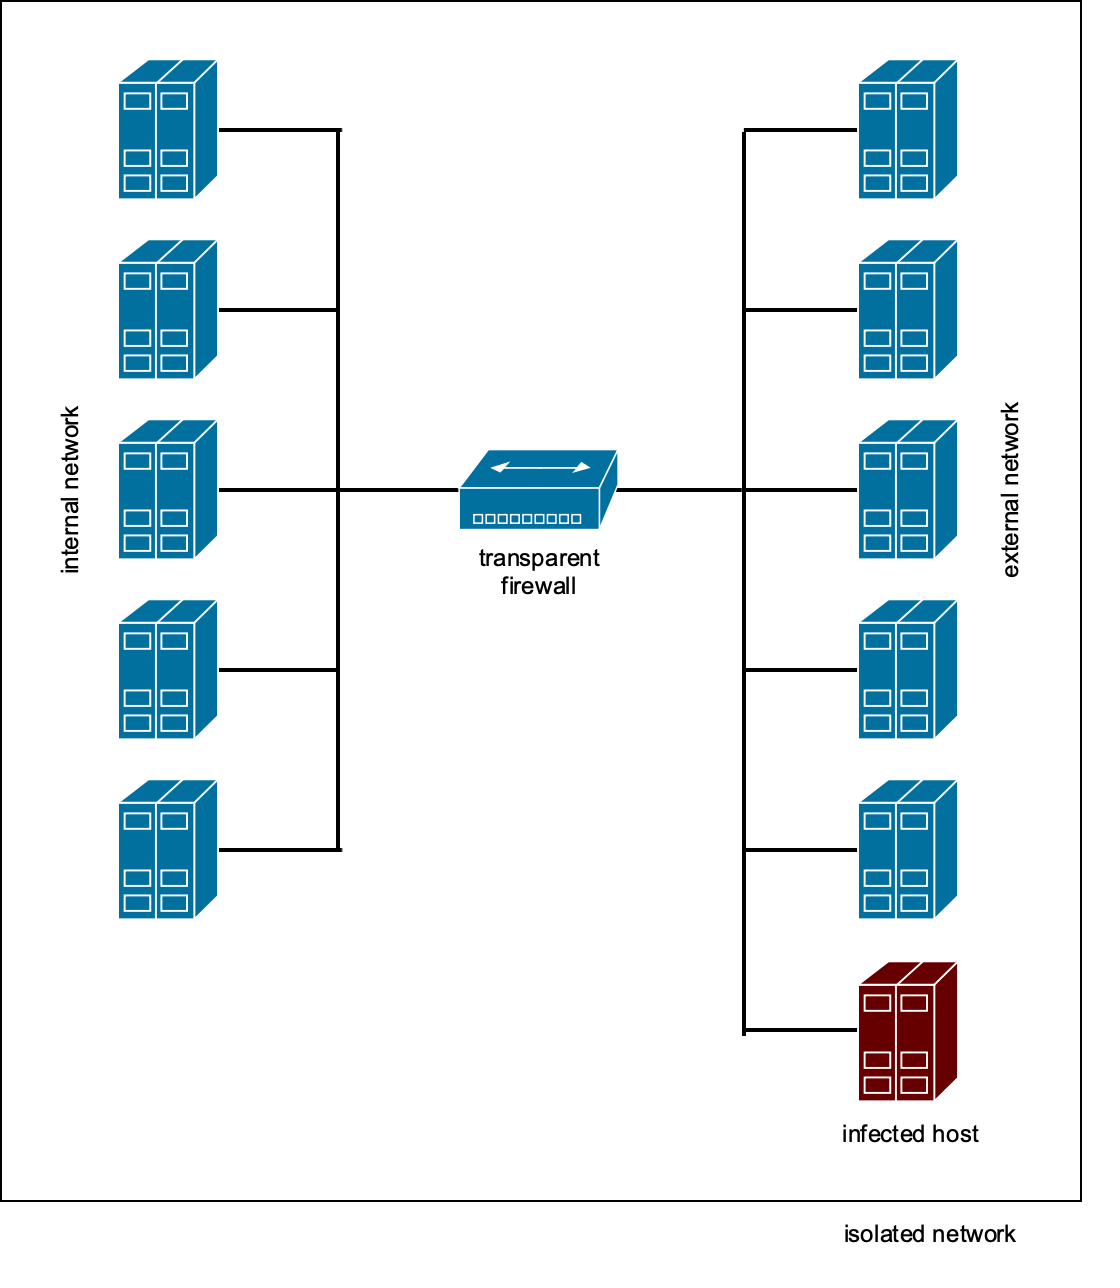
\includegraphics[width=200px]{resources/skenario_pengujian.png}
	\caption{Susunan jaringan skenario pengujian}
	\label{fig:validation_scenario}
\end{figure}

\section{Hasil Pengujian}

Data dari hasil percobaan berbentuk file pcap (\textit{packet capture}) dilakukan pengolahan untuk mendapatkan perkiraan waktu host terinfeksi. Hasil pengolahan data dapat dilihat di Lampiran B berisi data perkiraan waktu host terinfeksi. Kemudian data tersebut diakumulasikan untuk setiap percobaan untuk mendapatkan data pada suatu waktu telah ada berapa host terinfeksi.

\begin{figure}[H]
	\centering
	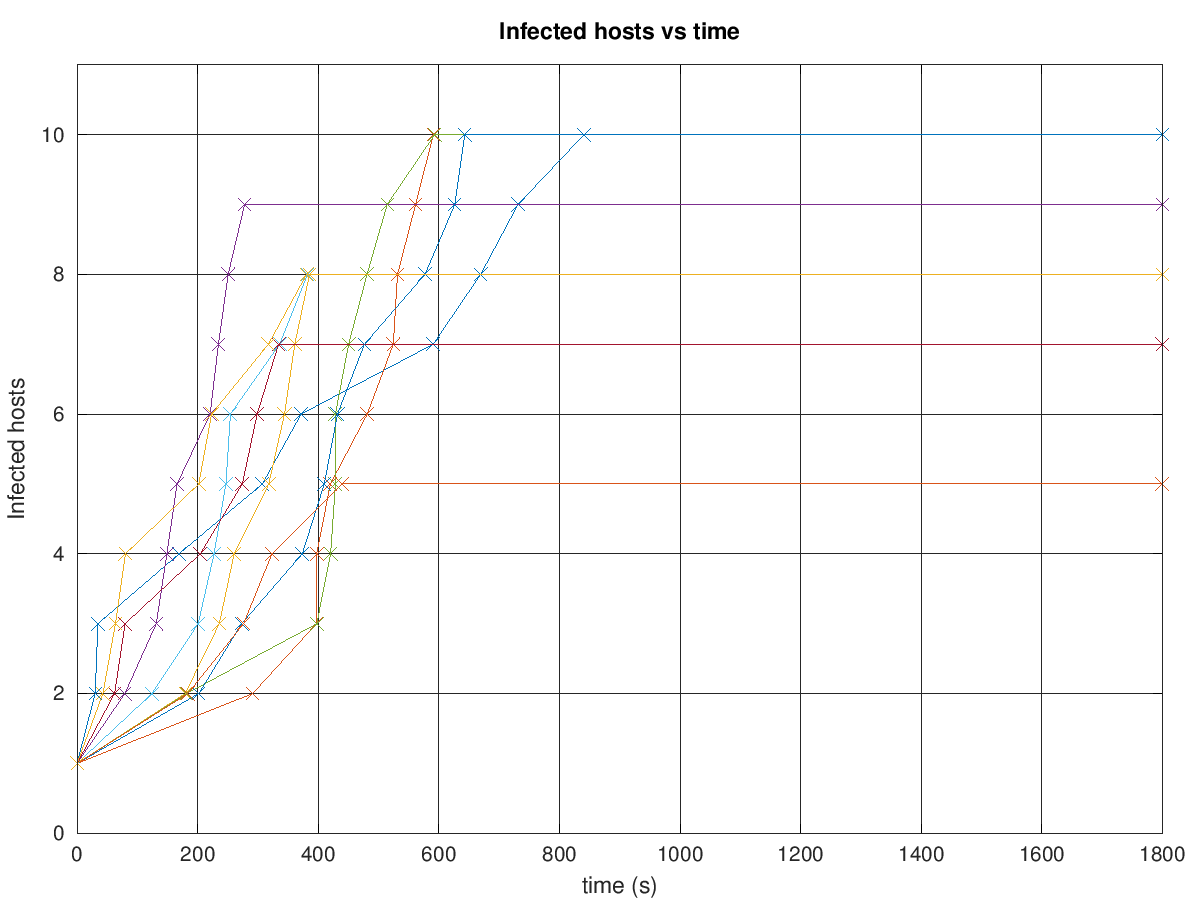
\includegraphics[width=\textwidth]{resources/infection_control_over_time.png}
	\caption{Grafik host terinfeksi terhadap waktu (percobaan kontrol)}
	\label{fig:infection_control_over_time}
\end{figure}

Grafik akumulasi host terinfeksi pada percobaan kontrol dapat dilihat pada gambar \ref{fig:infection_control_over_time}. Grafik tersebut berisi 10 data percobaan kontrol. Dari 10 percobaan tersebut dapat diperkirakan setelah 900 detik sudah terdapat lebih dari 5 host terinfeksi baik dari \textit{internal\_network} maupun \textit{external\_network}.

\begin{table}[H]
	\caption{Akumulasi detik ke-1800 host terinfeksi (percobaan kontrol)}
	\label{table:1800s_all_network_control}
	\begin{center}
		\begin{tabularx}{300px}{|X|r|}
			\hline
			\multicolumn{1}{|l}{\textbf{Jumlah host terinfeksi}} & \multicolumn{1}{|l|}{\textbf{teramati}} \\ \hline
			5 & 1 percobaan\\ \hline
			7 & 1 percobaan\\ \hline
			8 & 3 percobaan\\ \hline
			9 & 1 percobaan\\ \hline
			10 & 4 percobaan\\ \hline
		\end{tabularx}
	\end{center}
\end{table}

\begin{table}[H]
	\caption{Akumulasi detik ke-1800 host \textit{internal\_network} terinfeksi (percobaan kontrol)}
	\label{table:1800s_internal_network_control}
	\begin{center}
		\begin{tabularx}{300px}{|X|r|}
			\hline
			\multicolumn{1}{|l}{\textbf{Jumlah host \textit{internal\_network} terinfeksi}} & \multicolumn{1}{|l|}{\textbf{teramati}} \\ \hline
			2 & 1 percobaan\\ \hline
			3 & 1 percobaan\\ \hline
			4 & 4 percobaan\\ \hline
			5 & 4 percobaan\\ \hline
		\end{tabularx}
	\end{center}
\end{table}

Pada tabel \ref{table:1800s_all_network_control} dapat dilihat persebaran hasil pengamatan host terinfeksi pada \textit{internal\_network} maupun \textit{external\_network}. Sedangkan pada tabel \ref{table:1800s_internal_network_control} dapat dilihat persebaran pengamatan host terinfeksi pada \textit{internal\_network}. Kedua distribusi ini dapat menggambarkan perilaku infeksi WannaCry.

\begin{table}[H]
	\caption{Akumulasi detik ke-1800 host terinfeksi (percobaan firewall implementasi)}
	\label{table:1800s_all_network_firewalled}
	\begin{center}
		\begin{tabularx}{300px}{|X|r|}
			\hline
			\multicolumn{1}{|l}{\textbf{Jumlah host terinfeksi}} & \multicolumn{1}{|l|}{\textbf{teramati}} \\ \hline
			1 & 40 percobaan\\ \hline
			2 & 15 percobaan\\ \hline
			3 & 16 percobaan\\ \hline
			4 & 3 percobaan\\ \hline
			5 & 8 percobaan\\ \hline
			4 & 1 percobaan\\ \hline
		\end{tabularx}
	\end{center}
\end{table}

\begin{figure}[H]
	\centering
	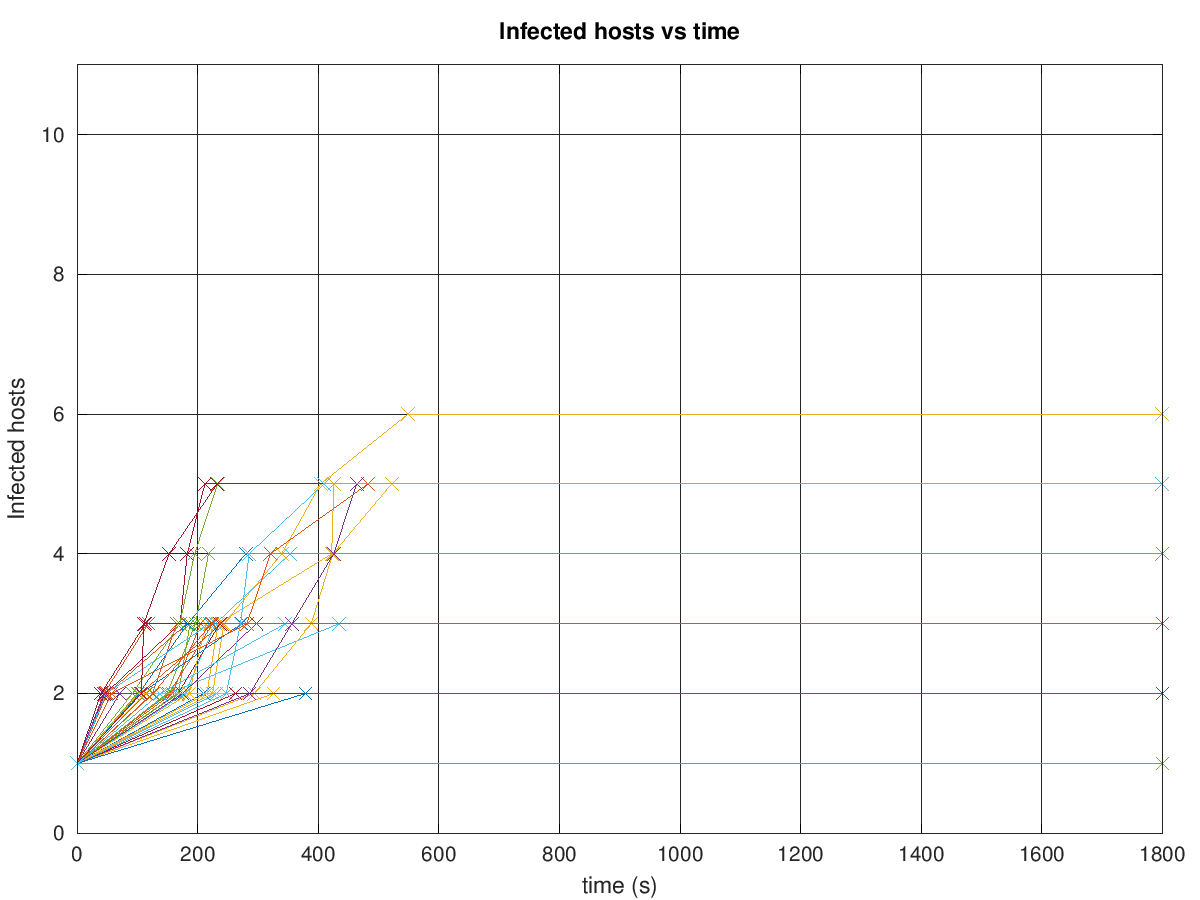
\includegraphics[width=\textwidth]{resources/infection_control_over_time_firewalled.png}
	\caption{Grafik host terinfeksi terhadap waktu (percobaan implementasi firewall)}
	\label{fig:infection_control_over_time_firewalled}
\end{figure}

Grafik akumulasi host teinfeksi pada percobaan implementasi firewall dapat dilihat pada gambar \ref{fig:infection_control_over_time_firewalled}. Pada gambar tersebut diamati setelah detik ke-600 tidak terjadi infeksi. Jumlah maksimum infeksi yang terjadi sebanyak 6 host yakni host pada \textit{external\_network}. Persebaran pengamatan host terinfeksi pada keseluruhan network dapat dilihat pada tabel \ref{table:1800s_all_network_firewalled}. Dari 83 percobaan tidak diamati infeksi terjadi pada \textit{internal\_network}.

\section{Pembahasan}

Pada subbab ini dijelaskan bagaimana tujuan pada bab I berhasil dilakukan berdasarkan data yang didapatkan pada percobaan. Selain itu dalam subbab ini dijelaskan kelemahan dan kemungkinan pengembangan selanjutnya. Kelemahan dan kemungkinan pengembangan selanjutnya yang kemudian disimpulkan dalam bab selanjutnya.

Percobaan kontrol menjadi dasar untuk membuktikan bahwa tujuan tercapai. Percobaan kontrol menunjukan bahwa malware WannaCry tetap dapat menginfeksi meskipun melalui sebuah bridge, dalam hal ini juga berlaku sebagai transparent firewall namun belum diterapkan rule. Percobaan ini menunjukan dengan kondisi tanpa perlakuan WannaCry dapat menginfeksi \textit{internal\_network}. Jika implementasi dapat mencapai tujuan, maka dengan perlakuan tersebut seharusnya WannaCry tidak dapat menginfeksi \textit{internal\_network}.

Kemudian hasil percobaan firewall implementasi dari 83 data yang diamati, tidak terjadi infeksi pada \textit{internal\_network}. Sehingga dapat disimpulkan tujuan yang disampaikan pada bab I tercapai. Dari 83 data masih belum diamati \textit{false-negative}. \textit{False-negative} seharusnya dapat diamati ketika terjadi infeksi pada \textit{internal\_network}. Kemudian dari packet capture yang dilakukan dapat dilakukan analisis.

Selain itu \textit{false-positive} juga sulit diamati dari data tersebut karena pengujian hanya memperhatikan bagaimana infeksi terjadi. Sedangkan tidak melakukan pengecekan pada protokol SMB pada keadaan normal. Walaupun penulis telah melakukan pengujian pada saat implementasi, dan mengamati bahwa rule firewall tersebut tidak mengganggu proses normal.

Bagian menarik dari data pada Lampiran B, malware ini tidak menginfeksi \textit{external\_network} secara maksimal ketika rule diterapkan. Dari hal ini dapat ditarik sebuah kesimpulan ketika malware ditangani pada suatu sisi, sisi lain dari network pun menjadi lebih aman. Hal ini terjadi karena \textit{internal\_network} tidak menjadi host yang terinfeksi dan kemudian ikut menyerang host lain.

Implementasi dalam bentuk \textit{signature-based} memiliki kelebihan untuk dapat menangkap signature dengan tingkat \textit{false-negative} yang kecil. Implementasi pada iptables merupakan bentuk implementasi \textit{realtime dynamic signature-based detection}. Implementasi DPI dalam bentuk ini perlu memperhatikan fragmentasi paket, sehingga paket perlu ditunggu hingga lengkap untuk dapat dianalisis. Pada implementasi saat ini masih belum secara detail diperhatikan, sehingga memungkinkan untuk menimbulkan false-negative.

Pada pengembangan selanjutnya, seharusnya implementasi dalam bentuk ini dapat digunakan untuk mendeteksi signature malware-malware yang telah diketahui. Hal ini seharusnya dapat menekan \textit{long-tail infection} yang tejadi seperti pada malware WannaCry ini. Namun, tidak semua malware dapat dideteksi dengan implementasi ini. Hal ini karena tidak semua signature infeksi dapat ditemukan dalam satu koneksi seperti yang terjadi pada WannaCry. Oleh karena itu diperlukan implementasi state-machine yang tidak hanya \textit{single-connection oriented}.

\chapter{Penutup}

Pada bab ini disampaikan kesimpulan yang didapatkan dari tugas akhir ini. Kemudian bab ini dilanjutkan dengan saran dari penulis.

\section{Kesimpulan}

Implementasi DPI pada firewall open-source iptables dapat digunakan sebagai penangkal malware yang pada tugas akhir ini dibatasi pada malware WannaCry. Implementasi dilakukan dengan menggunakan teknik \textit{dynamic signature-based}. Pengujian yang dilakukan belum ditemukan \textit{false-negative} pada implementasi DPI ini.

\section{Saran}

Saran-saran untuk pengembangan selanjutnya berdasarkan pengembangan yang telah dilakukan.
\begin{enumerate}
	\item Membuat \textit{Domain Specific Language} untuk merepresentasikan sebuah protokol. Dengan DSL diharapkan penambahan jenis protokol untuk DPI dapat dilakukan dengan lebih mudah.
	\item Implementasi \textit{state machine} yang tidak hanya bergantung pada satu koneksi. Hal ini dapat meningkatkan kemampuan firewall untuk mendeteksi malware yang melakukan infeksi tidak hanya menggunakan \textit{single-connection}.
	\item Implementasi \textit{Deep Packet Inspection} yang memperhatikan performa.
\end{enumerate}


\printbibliography

\appendix
\addcontentsline{toc}{part}{Lampiran}
\part*{Lampiran}

\chapter{Instrumen Pengujian}

Lampiran ini berisi instrumen pengujian yang digunakan untuk melakukan pengumpulan data. Pengumpulan data dilakukan dengan otomasi pada \textit{hypervisor} yang menggunakan \verb|qemu|. Otomasi dilakukan untuk mengumpulkan data dalam bentuk \verb|pcap|. Lampiran ini ditambahkan untuk mempermudah pembaca untuk mendapatkan data seperti yang dilakukan pada penelitian ini.

\section{Konfigurasi}

Dalam instrumen pengujian yang digunakan untuk pengumpulan data terdapat beberapa konfigurasi penting, yakni: bridge, dhcp server dan transparent firewall.

\subsection{/etc/dhcp/dhcpd.conf}

\begin{lstlisting}
option domain-name "local";
option domain-name-servers dhcp.local;
default-lease-time 600;
max-lease-time 7200;
authoritative;

subnet 192.168.1.0 netmask 255.255.255.0 {
	range dynamic-bootp 192.168.1.100 192.168.1.254;
	option broadcast-address 192.168.1.255;
	option routers 192.168.1.1;
}
\end{lstlisting}

\subsection{/etc/sysconfig/network-scripts/ifcfg-br0}

\begin{lstlisting}
DEVICE=br0
TYPE=Bridge
IPADDR=192.168.1.1
NETMASK=255.255.255.0
ONBOOT=yes
BOOTPROTO=none
NM_CONTROLLED=no
DELAY=0
\end{lstlisting}

\subsection{/etc/sysconfig/network-scripts/ifcfg-eth0}

\begin{lstlisting}
TYPE=Ethernet
DEVICE=eth0
BOOTPROTO=none
ONBOOT=yes
NM_CONTROLLED=no
BRIDGE=br0
\end{lstlisting}

\subsection{/etc/sysconfig/network-scripts/ifcfg-eth1}

\begin{lstlisting}
TYPE=Ethernet
DEVICE=eth1
BOOTPROTO=none
ONBOOT=yes
NM_CONTROLLED=no
BRIDGE=br0
\end{lstlisting}

\subsection{Konfigurasi Khusus Transparent Firewall}

\begin{lstlisting}
echo 1 > /proc/sys/net/bridge/bridge-nf-call-iptables
\end{lstlisting}

\section{Otomasi}

\subsection{start.sh}

Script ini digunakan untuk melakukan otomasi untuk menghidupkan \textit{instance virtual machine}, mengirimkan perintah capture, menghentikan \textit{instance virtual machine} dan mengatur kembali keadaan \textit{instance virtual machine}. Menghidupkan dan menghentikan instance virtual machine dilakukan dengan perintah \verb|virsh|. Mengirimkan perintah capture dengan melakukan \verb|SSH| ke firewall. Bagian mengatur kembali keadaan dengan menghapus image, dan menyalin dari master.

\begin{lstlisting}[language=Bash]
#!/bin/bash
echo "starting..."
for i in `seq 1 10`; do virsh start ibrohim-winsrv-$i; done;
echo "done."

sleep 5m;
ssh root@167.205.3.202 "screen -dm bash capture.sh"
sleep 1m;

virsh start ibrohim-wannacry-1
sleep 30m;
virsh destroy ibrohim-wannacry-1

echo "stopping..."
for i in `seq 1 10`; do virsh destroy ibrohim-winsrv-$i; done;
echo "done."

echo "cleanup..."
for i in `seq 1 10`; do rm -vf ibrohim-winsrv-$i.img; done;
rm -vf ibrohim-wannacry.img
echo "done."

echo "cloning..."
for i in `seq 1 10`; do cp -v ibrohim-winsrv-master.img ibrohim-winsrv-$i.img; done;
cp -v ibrohim-wannacry-master.img ibrohim-wannacry.img
echo "done."
\end{lstlisting}

\subsection{capture.sh}

Script ini digunakan untuk melakukan \textit{packet capture}. \textit{Packet capture} dilakukan dengan menggunakan perintah \verb|tcpdump|.

\begin{lstlisting}[language=Bash]
#!/bin/bash
i="1"
while [ -f output.$i.pcap ]; do let "i++"; done;
touch output.$i.pcap

file=output.$i.pcap

echo "output: $file"
echo "start capturing..."
tcpdump -s0 -vv -w $file &
sleep 30m; kill $!hmm

echo "done."
\end{lstlisting}


\chapter{Data Percobaan}

Lampiran ini berisi data hasil pemrosesan dari pcap yang didapatkan. Data berupa waktu relatif infeksi setelah host terinfeksi aktif. Tidak semua data dapat disajikan pada lampiran ini.

\section{Data Percobaan Kontrol}

Pada bagian ini disajikan data percobaan 1-10 dari percobaan kontrol yang dilakukan. Data dapat dilihat pada tabel \ref{table:data percobaan kontrol 1_4}, \ref{table:data percobaan kontrol 5_8}, dan \ref{table:data percobaan kontrol 9_10}.

\begin{table}[H]
	\caption{tabel data percobaan kontrol 1-4}
	\label{table:data percobaan kontrol 1_4}
	\centering
	\footnotesize
	\begin{tabular}{|l|l|l|l|l|}
		\hline
		\multirow{2}{*}{Mac Address} & \multicolumn{4}{c|}{Waktu relatif infeksi terdeteksi (detik)} \\ \cline{2-5} 
		& percobaan 1 & percobaan 2 & percobaan 3 & percobaan 4\\ \hline
		\verb|52:54:00:8a:d6:60| & 34.52585006 & 531.3917201 &  & 260.5722001 \\ \hline
		\verb|52:54:00:05:0f:b0| & 30.01635003 & 481.29196 & 223.1153898 &  \\ \hline
		\verb|52:54:00:53:55:f8| &  & 397.0566101 & 380.73404 &  \\ \hline
		\verb|52:54:00:94:47:8f| & 840.8641901 & 291.2939601 & 1696.60498 & 317.81583 \\ \hline
		\verb|52:54:00:4a:9b:54| & 169.0511401 & 420.2032199 &  & 179.34624 \\ \hline
		\verb|52:54:00:00:e4:8a| & 590.72333 & 524.4521599 & 317.41592 &  \\ \hline
		\verb|52:54:00:e4:6a:37| & 307.09745 & 397.28951 & 42.87851 & 235.8482299 \\ \hline
		\verb|52:54:00:5b:e8:4e| & 669.48561 &  & 63.50870991 & 344.0081699 \\ \hline
		\verb|52:54:00:0e:a5:bb| & 731.34987 & 561.53285 & 201.8673599 & 361.1401999 \\ \hline
		\verb|52:54:00:9e:a7:84| & 371.72616 & 590.89149 & 80.14567995 & 385.5174999 \\ \hline
		\verb|52:54:00:e2:b8:bf| & 0 & 0 & 0 & 0 \\ \hline
	\end{tabular}
\end{table}
\begin{table}[H]
	\caption{tabel data percobaan kontrol 5-8}
	\label{table:data percobaan kontrol 5_8}
	\centering
	\footnotesize
	\begin{tabular}{|l|l|l|l|l|}
		\hline
		\multirow{2}{*}{Mac Address} & \multicolumn{4}{c|}{Waktu relatif infeksi terdeteksi (detik)} \\ \cline{2-5} 
		& percobaan 5 & percobaan 6 & percobaan 7 & percobaan 8\\ \hline
		\footnotesize{\verb|52:54:00:8a:d6:60|} &  & 397.47768 & 246.9578202 & 62.15236998 \\ \hline
		\footnotesize{\verb|52:54:00:05:0f:b0|} & 234.4498501 & 593.17661 &  &  \\ \hline
		\footnotesize{\verb|52:54:00:53:55:f8|} & 165.7816901 & 181.5601101 &  & 334.0565798 \\ \hline
		\footnotesize{\verb|52:54:00:94:47:8f|} & 79.3713901 & 450.4038 & 227.1313701 & 273.9240201 \\ \hline
		\footnotesize{\verb|52:54:00:4a:9b:54|} &  & 480.8952699 & 335.96135 &  \\ \hline
		\footnotesize{\verb|52:54:00:00:e4:8a|} & 131.33215 &  & 124.2107902 & 298.6877699 \\ \hline
		\footnotesize{\verb|52:54:00:e4:6a:37|} & 220.54354 & 428.4335399 &  & 79.69015002 \\ \hline
		\footnotesize{\verb|52:54:00:5b:e8:4e|} & 277.8082199 & 428.4335399 & 382.1870301 & 204.14782 \\ \hline
		\footnotesize{\verb|52:54:00:0e:a5:bb|} & 250.7147601 & 420.5615299 & 254.2904701 &  \\ \hline
		\footnotesize{\verb|52:54:00:9e:a7:84|} & 148.8434501 & 514.30985 & 200.7130902 &  \\ \hline
		\footnotesize{\verb|52:54:00:e2:b8:bf|} & 0 & 0 & 0 & 0 \\ \hline
	\end{tabular}
\end{table}
\begin{table}[H]
	\caption{tabel data percobaan kontrol 9-10}
	\label{table:data percobaan kontrol 9_10}
	\centering
	\footnotesize
	\begin{tabular}{|l|l|l|}
		\hline
		\multirow{2}{*}{Mac Address} & \multicolumn{2}{c|}{Waktu relatif infeksi terdeteksi (detik)} \\ \cline{2-3} 
		& percobaan 9 & percobaan 10 \\ \hline
		\footnotesize{\verb|52:54:00:8a:d6:60|} & 643.0479999 & 276.06352 \\ \hline
		\footnotesize{\verb|52:54:00:05:0f:b0|} & 373.4961998 &  \\ \hline
		\footnotesize{\verb|52:54:00:53:55:f8|} & 577.2704098 & 183.78249 \\ \hline
		\footnotesize{\verb|52:54:00:94:47:8f|} &  &  \\ \hline
		\footnotesize{\verb|52:54:00:4a:9b:54|} & 201.7124 &  \\ \hline
		\footnotesize{\verb|52:54:00:00:e4:8a|} & 431.8800199 & 323.1868999 \\ \hline
		\footnotesize{\verb|52:54:00:e4:6a:37|} & 273.01895 & 439.2264998 \\ \hline
		\footnotesize{\verb|52:54:00:5b:e8:4e|} & 476.6982899 &  \\ \hline
		\footnotesize{\verb|52:54:00:0e:a5:bb|} & 626.4096398 &  \\ \hline
		\footnotesize{\verb|52:54:00:9e:a7:84|} & 410.0081699 &  \\ \hline
		\footnotesize{\verb|52:54:00:e2:b8:bf|} & 0 & 0 \\ \hline
	\end{tabular}
\end{table}

\pagebreak

\section{Data Percobaan Implementasi Firewall}

\begin{table}[H]
	\caption{tabel data percobaan implementasi firewall 1-4}
	\label{table:data percobaan implementasi firewall 1_4}
	\centering
	\footnotesize
	\begin{tabular}{|l|l|l|l|l|}
		\hline
		\multirow{2}{*}{Mac Address} & \multicolumn{4}{c|}{Waktu relatif infeksi terdeteksi (detik)} \\ \cline{2-5} 
		& percobaan 1 & percobaan 2 & percobaan 3 & percobaan 4\\ \hline
		\footnotesize{\verb|52:54:00:8a:d6:60|} &  &  &  & \\ \hline
		\footnotesize{\verb|52:54:00:05:0f:b0|} &  & 182.1739399 & 325.7423799 & \\ \hline
		\footnotesize{\verb|52:54:00:53:55:f8|} &  &  &  & \\ \hline
		\footnotesize{\verb|52:54:00:94:47:8f|} &  &  &  & \\ \hline
		\footnotesize{\verb|52:54:00:4a:9b:54|} & 209.6183 & 49.69097996 &  & \\ \hline
		\footnotesize{\verb|52:54:00:00:e4:8a|} &  &  &  & \\ \hline
		\footnotesize{\verb|52:54:00:e4:6a:37|} &  &  &  & \\ \hline
		\footnotesize{\verb|52:54:00:5b:e8:4e|} &  &  &  & \\ \hline
		\footnotesize{\verb|52:54:00:0e:a5:bb|} &  &  &  & \\ \hline
		\footnotesize{\verb|52:54:00:9e:a7:84|} &  &  &  & \\ \hline
		\footnotesize{\verb|52:54:00:e2:b8:bf|} & 0 & 0 & 0 & 0\\ \hline
	\end{tabular}
\end{table}

\begin{table}[H]
	\caption{tabel data percobaan implementasi firewall 5-8}
	\label{table:data percobaan implementasi firewall 5_8}
	\centering
	\footnotesize
	\begin{tabular}{|l|l|l|l|l|}
		\hline
		\multirow{2}{*}{Mac Address} & \multicolumn{4}{c|}{Waktu relatif infeksi terdeteksi (detik)} \\ \cline{2-5} 
		& percobaan 5 & percobaan 6 & percobaan 7 & percobaan 8\\ \hline
		\footnotesize{\verb|52:54:00:8a:d6:60|} &  &  &  & \\ \hline
		\footnotesize{\verb|52:54:00:05:0f:b0|} &  &  &  & \\ \hline
		\footnotesize{\verb|52:54:00:53:55:f8|} &  & 178.27004 &  & \\ \hline
		\footnotesize{\verb|52:54:00:94:47:8f|} & 99.65812016 &  &  & \\ \hline
		\footnotesize{\verb|52:54:00:4a:9b:54|} &  &  &  & \\ \hline
		\footnotesize{\verb|52:54:00:00:e4:8a|} &  &  &  & \\ \hline
		\footnotesize{\verb|52:54:00:e4:6a:37|} &  &  &  & \\ \hline
		\footnotesize{\verb|52:54:00:5b:e8:4e|} &  &  &  & \\ \hline
		\footnotesize{\verb|52:54:00:0e:a5:bb|} &  &  &  & \\ \hline
		\footnotesize{\verb|52:54:00:9e:a7:84|} &  &  &  & \\ \hline
		\footnotesize{\verb|52:54:00:e2:b8:bf|} & 0 & 0 & 0 & 0\\ \hline
	\end{tabular}
\end{table}

\begin{table}[H]
	\caption{tabel data percobaan implementasi firewall 9-12}
	\label{table:data percobaan implementasi firewall 9_12}
	\centering
	\footnotesize
	\begin{tabular}{|l|l|l|l|l|}
		\hline
		\multirow{2}{*}{Mac Address} & \multicolumn{4}{c|}{Waktu relatif infeksi terdeteksi (detik)} \\ \cline{2-5} 
		& percobaan 9 & percobaan 10 & percobaan 11 & percobaan 12\\ \hline
		\footnotesize{\verb|52:54:00:8a:d6:60|} &  & 233.91587 &  & \\ \hline
		\footnotesize{\verb|52:54:00:05:0f:b0|} &  & 215.2593 &  & \\ \hline
		\footnotesize{\verb|52:54:00:53:55:f8|} & 204.8192298 &  &  & 126.7261798\\ \hline
		\footnotesize{\verb|52:54:00:94:47:8f|} & 157.9287698 & 422.3015499 &  & \\ \hline
		\footnotesize{\verb|52:54:00:4a:9b:54|} &  & 425.8468499 &  & \\ \hline
		\footnotesize{\verb|52:54:00:00:e4:8a|} &  &  &  & \\ \hline
		\footnotesize{\verb|52:54:00:e4:6a:37|} &  &  &  & \\ \hline
		\footnotesize{\verb|52:54:00:5b:e8:4e|} &  &  &  & \\ \hline
		\footnotesize{\verb|52:54:00:0e:a5:bb|} &  &  &  & \\ \hline
		\footnotesize{\verb|52:54:00:9e:a7:84|} &  &  &  & \\ \hline
		\footnotesize{\verb|52:54:00:e2:b8:bf|} & 0 & 0 & 0 & 0\\ \hline
	\end{tabular}
\end{table}

\begin{table}[H]
	\caption{tabel data percobaan implementasi firewall 13-16}
	\label{table:data percobaan implementasi firewall 13_16}
	\centering
	\footnotesize
	\begin{tabular}{|l|l|l|l|l|}
		\hline
		\multirow{2}{*}{Mac Address} & \multicolumn{4}{c|}{Waktu relatif infeksi terdeteksi (detik)} \\ \cline{2-5} 
		& percobaan 13 & percobaan 14 & percobaan 15 & percobaan 16\\ \hline
		\verb|52:54:00:8a:d6:60| &  & 182.61589 &  & \\ \hline
		\verb|52:54:00:05:0f:b0| &  &  &  & \\ \hline
		\verb|52:54:00:53:55:f8| &  & 46.83728004 &  & \\ \hline
		\verb|52:54:00:94:47:8f| &  & 212.0060401 &  & \\ \hline
		\verb|52:54:00:4a:9b:54| &  & 170.8900802 &  & \\ \hline
		\verb|52:54:00:00:e4:8a| &  &  &  & \\ \hline
		\verb|52:54:00:e4:6a:37| &  &  &  & \\ \hline
		\verb|52:54:00:5b:e8:4e| &  &  &  & \\ \hline
		\verb|52:54:00:0e:a5:bb| &  &  &  & \\ \hline
		\verb|52:54:00:9e:a7:84| &  &  &  & \\ \hline
		\verb|52:54:00:e2:b8:bf| & 0 & 0 & 0 & 0\\ \hline
	\end{tabular}
\end{table}


\end{document}
